\starredchapter{ANNEXE~\thechapter. FIGURES SUPPLÉMENTAIRES}\label{app:supp-figs}

\begin{figure}[htb]
    \centering
    \pdftooltip{\includegraphics[width=5in]{figs/supp_figs/August30,2007Prey241217.png}}{Figure \ref{fig:prey-samples-2007}}
    \caption{Emplacements et identité du stock (probabilité la plus élevée pour un échantillon donné) des restes de proies des ERSN récoltés le 30 août 2007.}
    \label{fig:prey-samples-2007}
\end{figure}

\begin{figure}[htb]
    \centering
    \pdftooltip{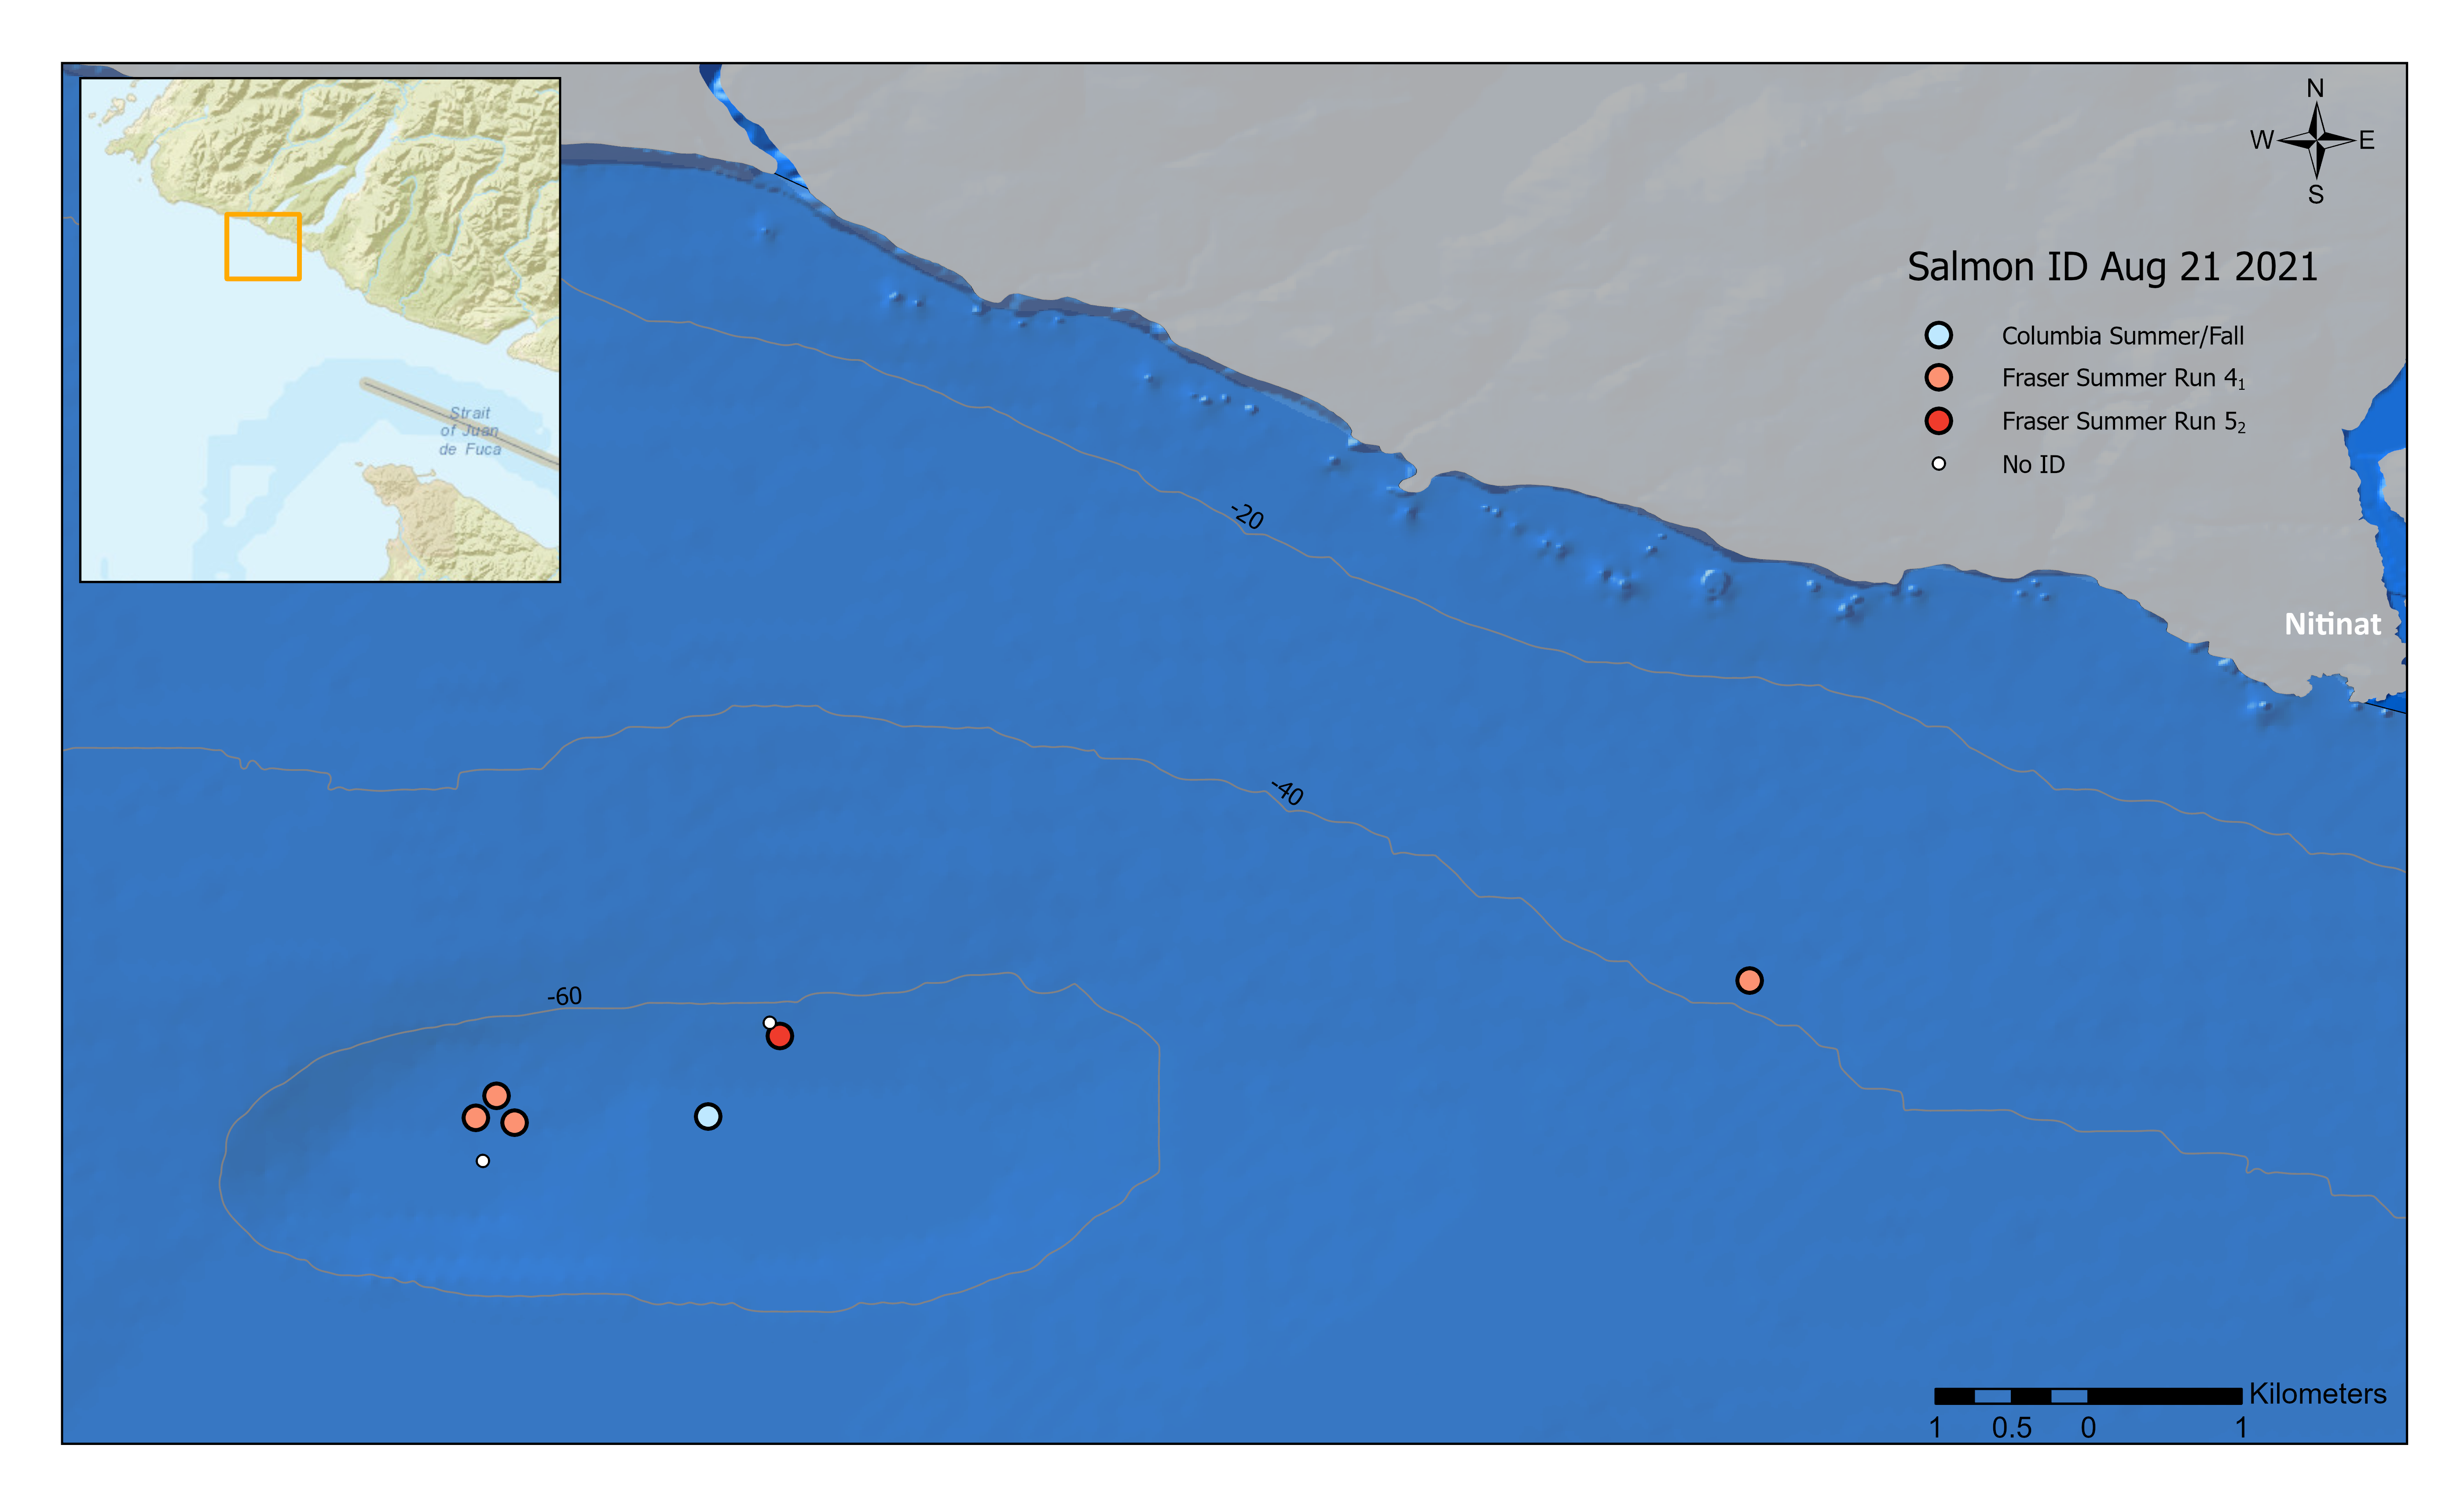
\includegraphics[width=5in]{figs/supp_figs/August21,2021Prey241217.png}}{Figure \ref{fig:prey-samples-2017}}
    \caption{Emplacements et identité du stock (probabilité la plus élevée pour un échantillon donné) des restes de proies des ERSN récoltés le 21 août 2017.}
    \label{fig:prey-samples-2017}
\end{figure}

\begin{figure}[htb]
    \centering
    \pdftooltip{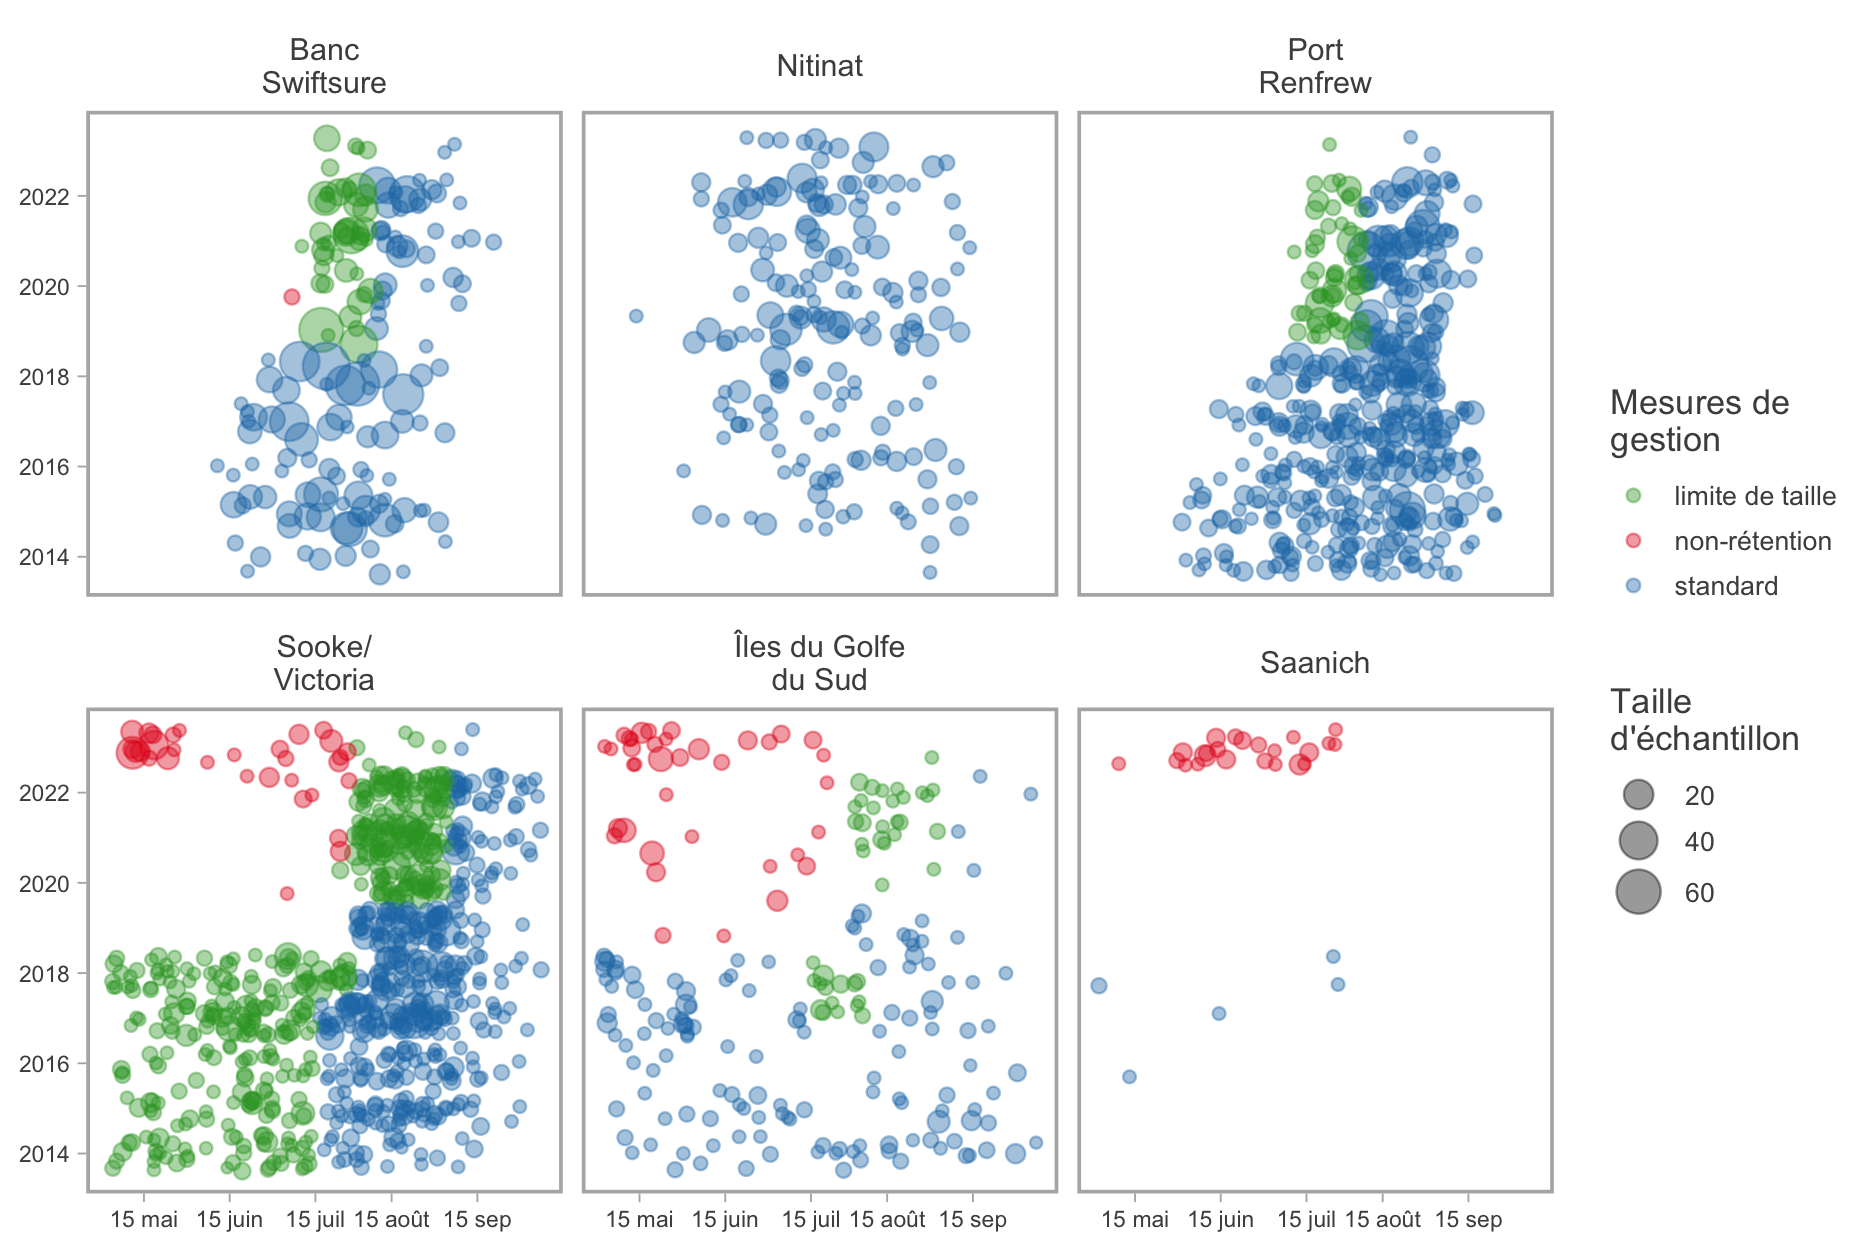
\includegraphics[width=5in]{figs/supp_figs/rec_temporal_sample_coverage_management.png}}{Figure \ref{fig:temporal-fishery-samples-management}}
    \caption{Distribution temporelle des échantillons de composition du stock de saumon chinook provenant des pêches récréatives entre mai et octobre, et mesures de gestion supplémentaires associées (couleurs). Les strates (panneaux) correspondent aux domaines spatiaux de la Figure \ref{fig:sampling-map}. Les échantillons prélevés pendant la non-rétention provenaient soit d'échantillons de pêcheurs passionnés de poissons remis à l'eau, soit de pêches de référence scientifiques. Notez que cette figure n'est pas destinée à saisir précisément les actions de gestion. Les limites de taille varient entre et à l'intérieur des strates et peuvent inclure à la fois des limites de taille minimale et maximale. Pour des informations détaillées sur les interventions spécifiques, consultez Dobson et al. 2020 pour les années antérieures à 2019 et les PGIP annuels (p. ex., MPO 2023). La taille des points est mise à l'échelle du nombre d'échantillons individuels collectés dans un lieu de pêche, une semaine et une année donnés. Les points ont été décalés pour maximiser la visibilité.}
    \label{fig:temporal-fishery-samples-management}
\end{figure}

\begin{figure}[htb]
    \centering
    \pdftooltip{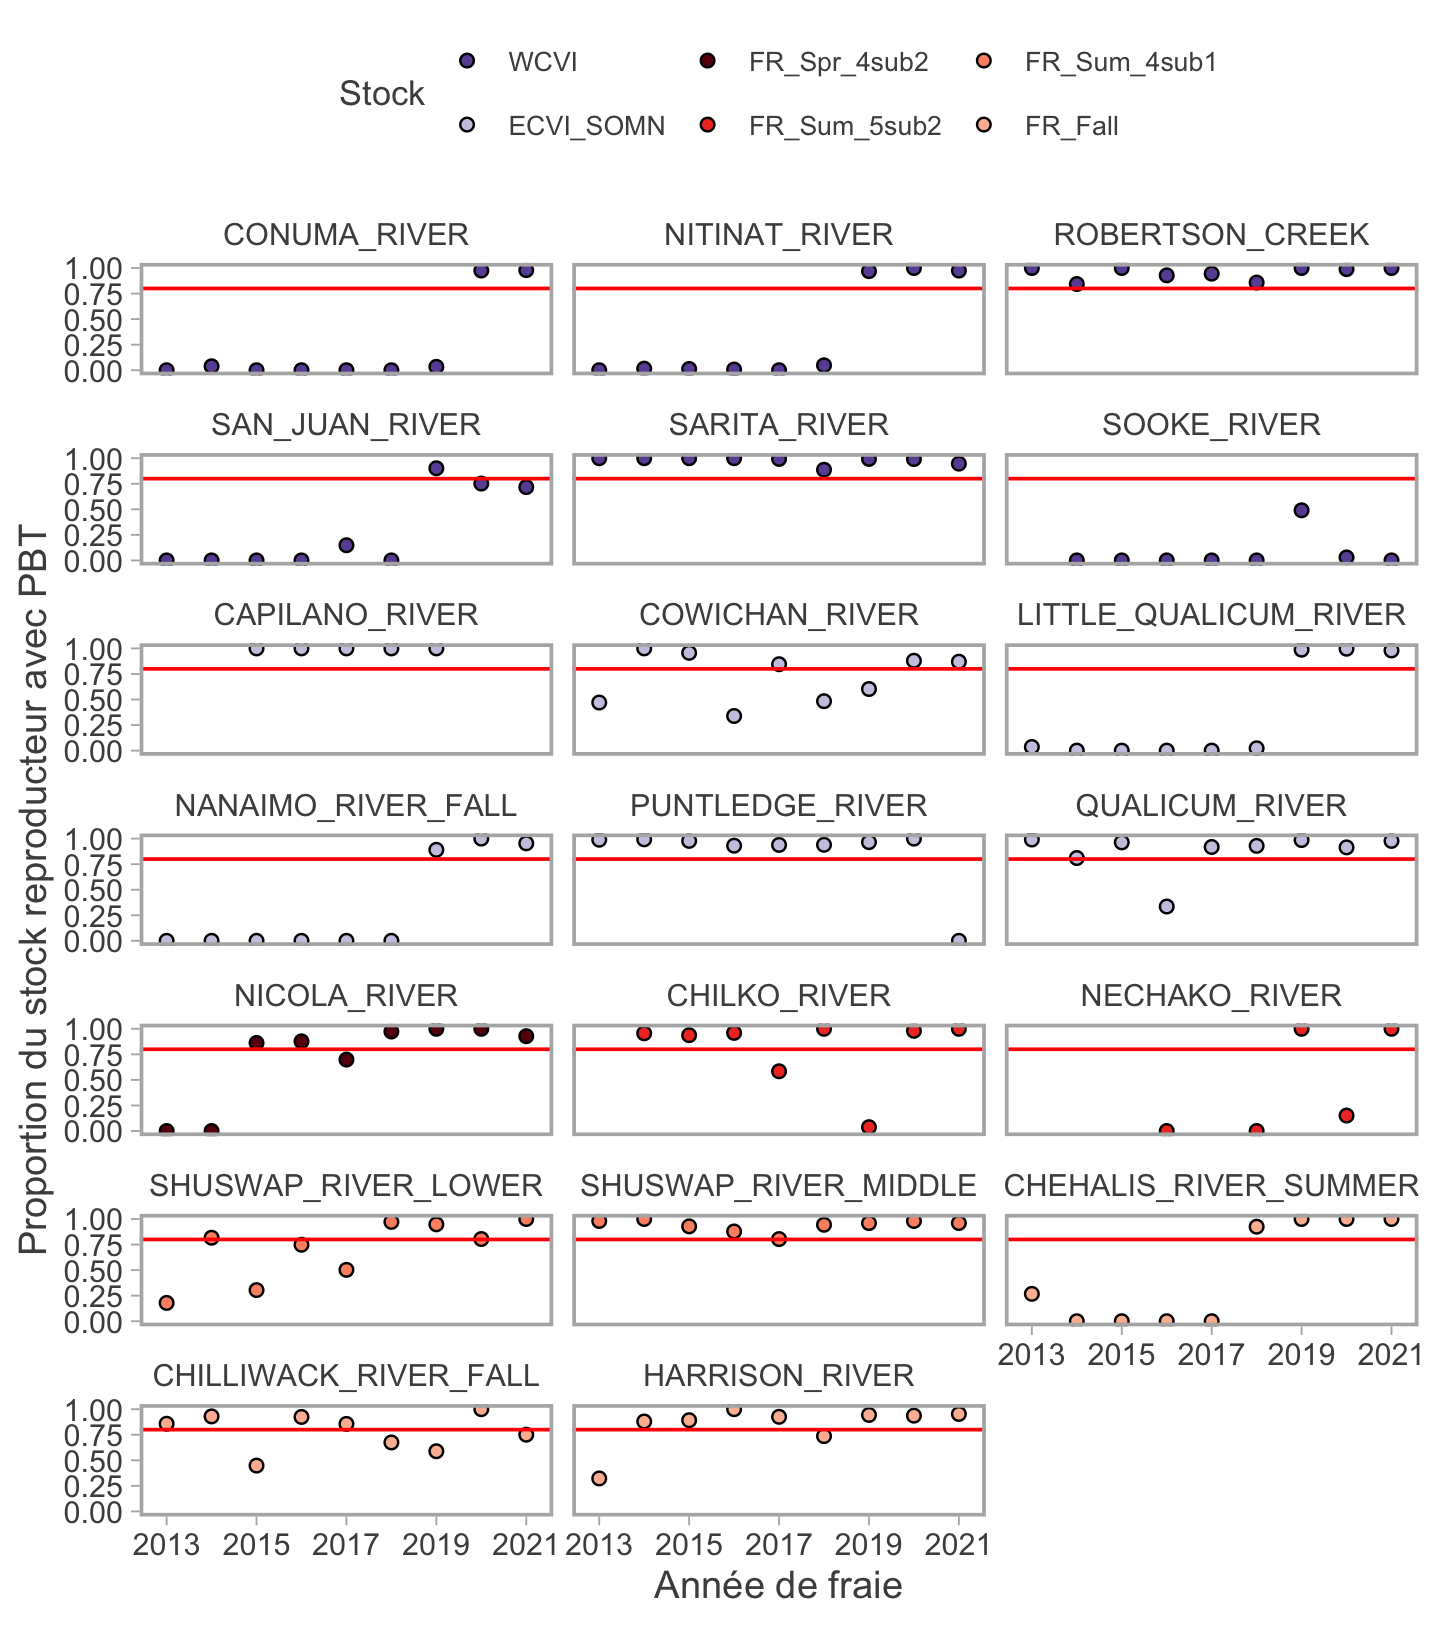
\includegraphics[width=5in]{figs/supp_figs/pbt_rate.png}}{Figure \ref{fig:pbt-coverage}}
    \caption{La proportion du stock géniteur de saumon chinook d'écloserie, par année de frai, incorporée dans la base de données EPF. La ligne rouge horizontale représente le seuil de marquage en deçà duquel les individus identifiés par GSI ont été assignés à une origine inconnue. Seules les principales installations d'amélioration (libérations annuelles moyennes supérieures à 140 000) avec des routes migratoires près de la zone d'étude sont présentées. Nechako et Chilko ont des tailles de libération annuelles moyennes inférieures à 140 000, mais sont présentées car les deux stocks étaient relativement abondants dans les pêches récréatives. Notez que les années de frai précèdent les années de retour d'au moins deux ans.}
    \label{fig:pbt-coverage}
\end{figure}

\begin{figure}[htb]
    \centering
    \pdftooltip{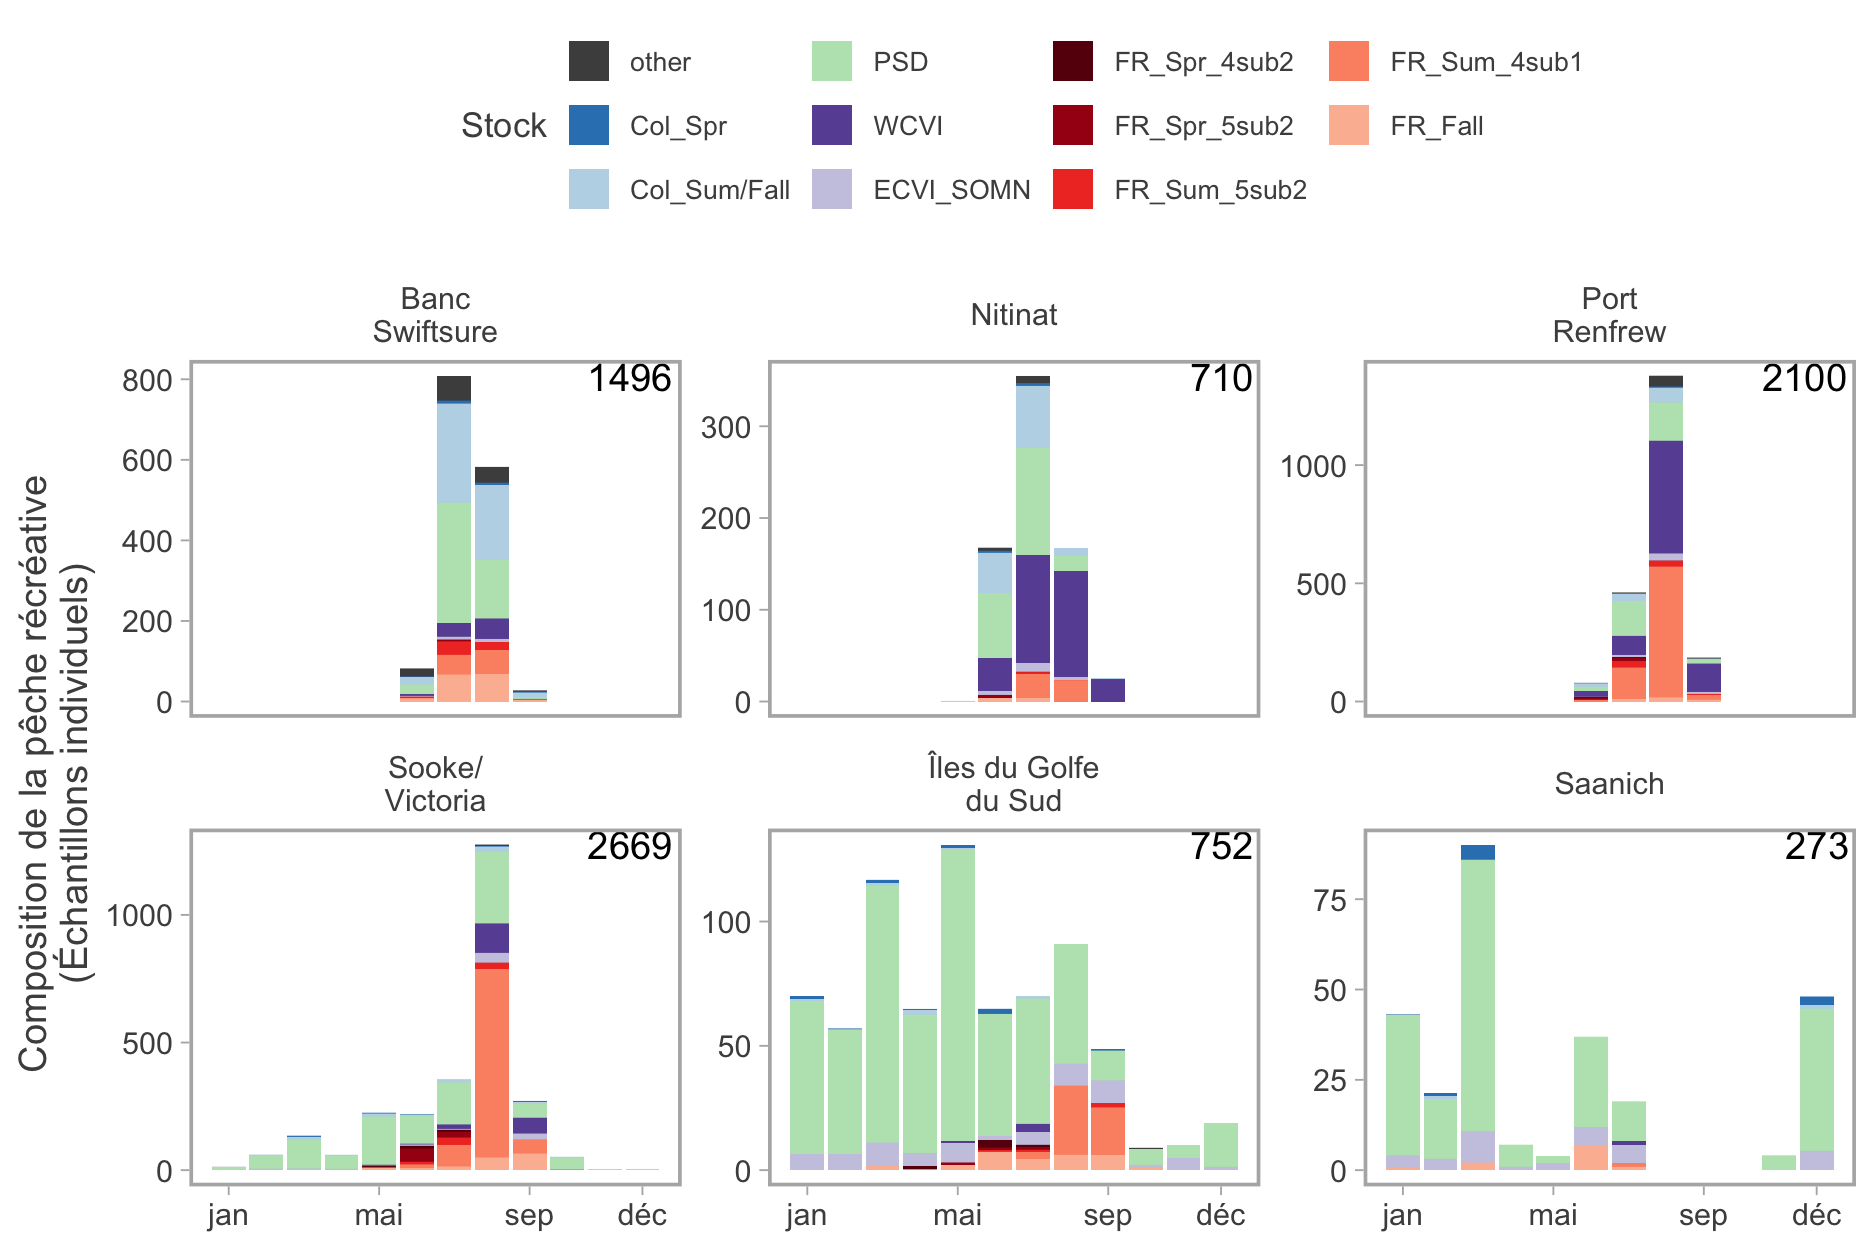
\includegraphics[width=5in]{figs/supp_figs/rec_monthly_comp_bar.png}}{Figure \ref{fig:bar-rec-full}}
    \caption{Composition mensuelle du stock d'échantillons de la pêche récréative de saumon chinook pendant tous les mois. Les strates (panneaux) correspondent aux domaines spatiaux de la Figure \ref{fig:sampling-map}. L'axe des y représente le nombre d'échantillons collectés dans un mois et une strate spatiale donnés. Les chiffres dans le coin supérieur droit de chaque panneau représentent la taille totale de l'échantillon dans chaque strate.}
    \label{fig:bar-rec-full}
\end{figure}

\begin{figure}[htb]
    \centering
    \pdftooltip{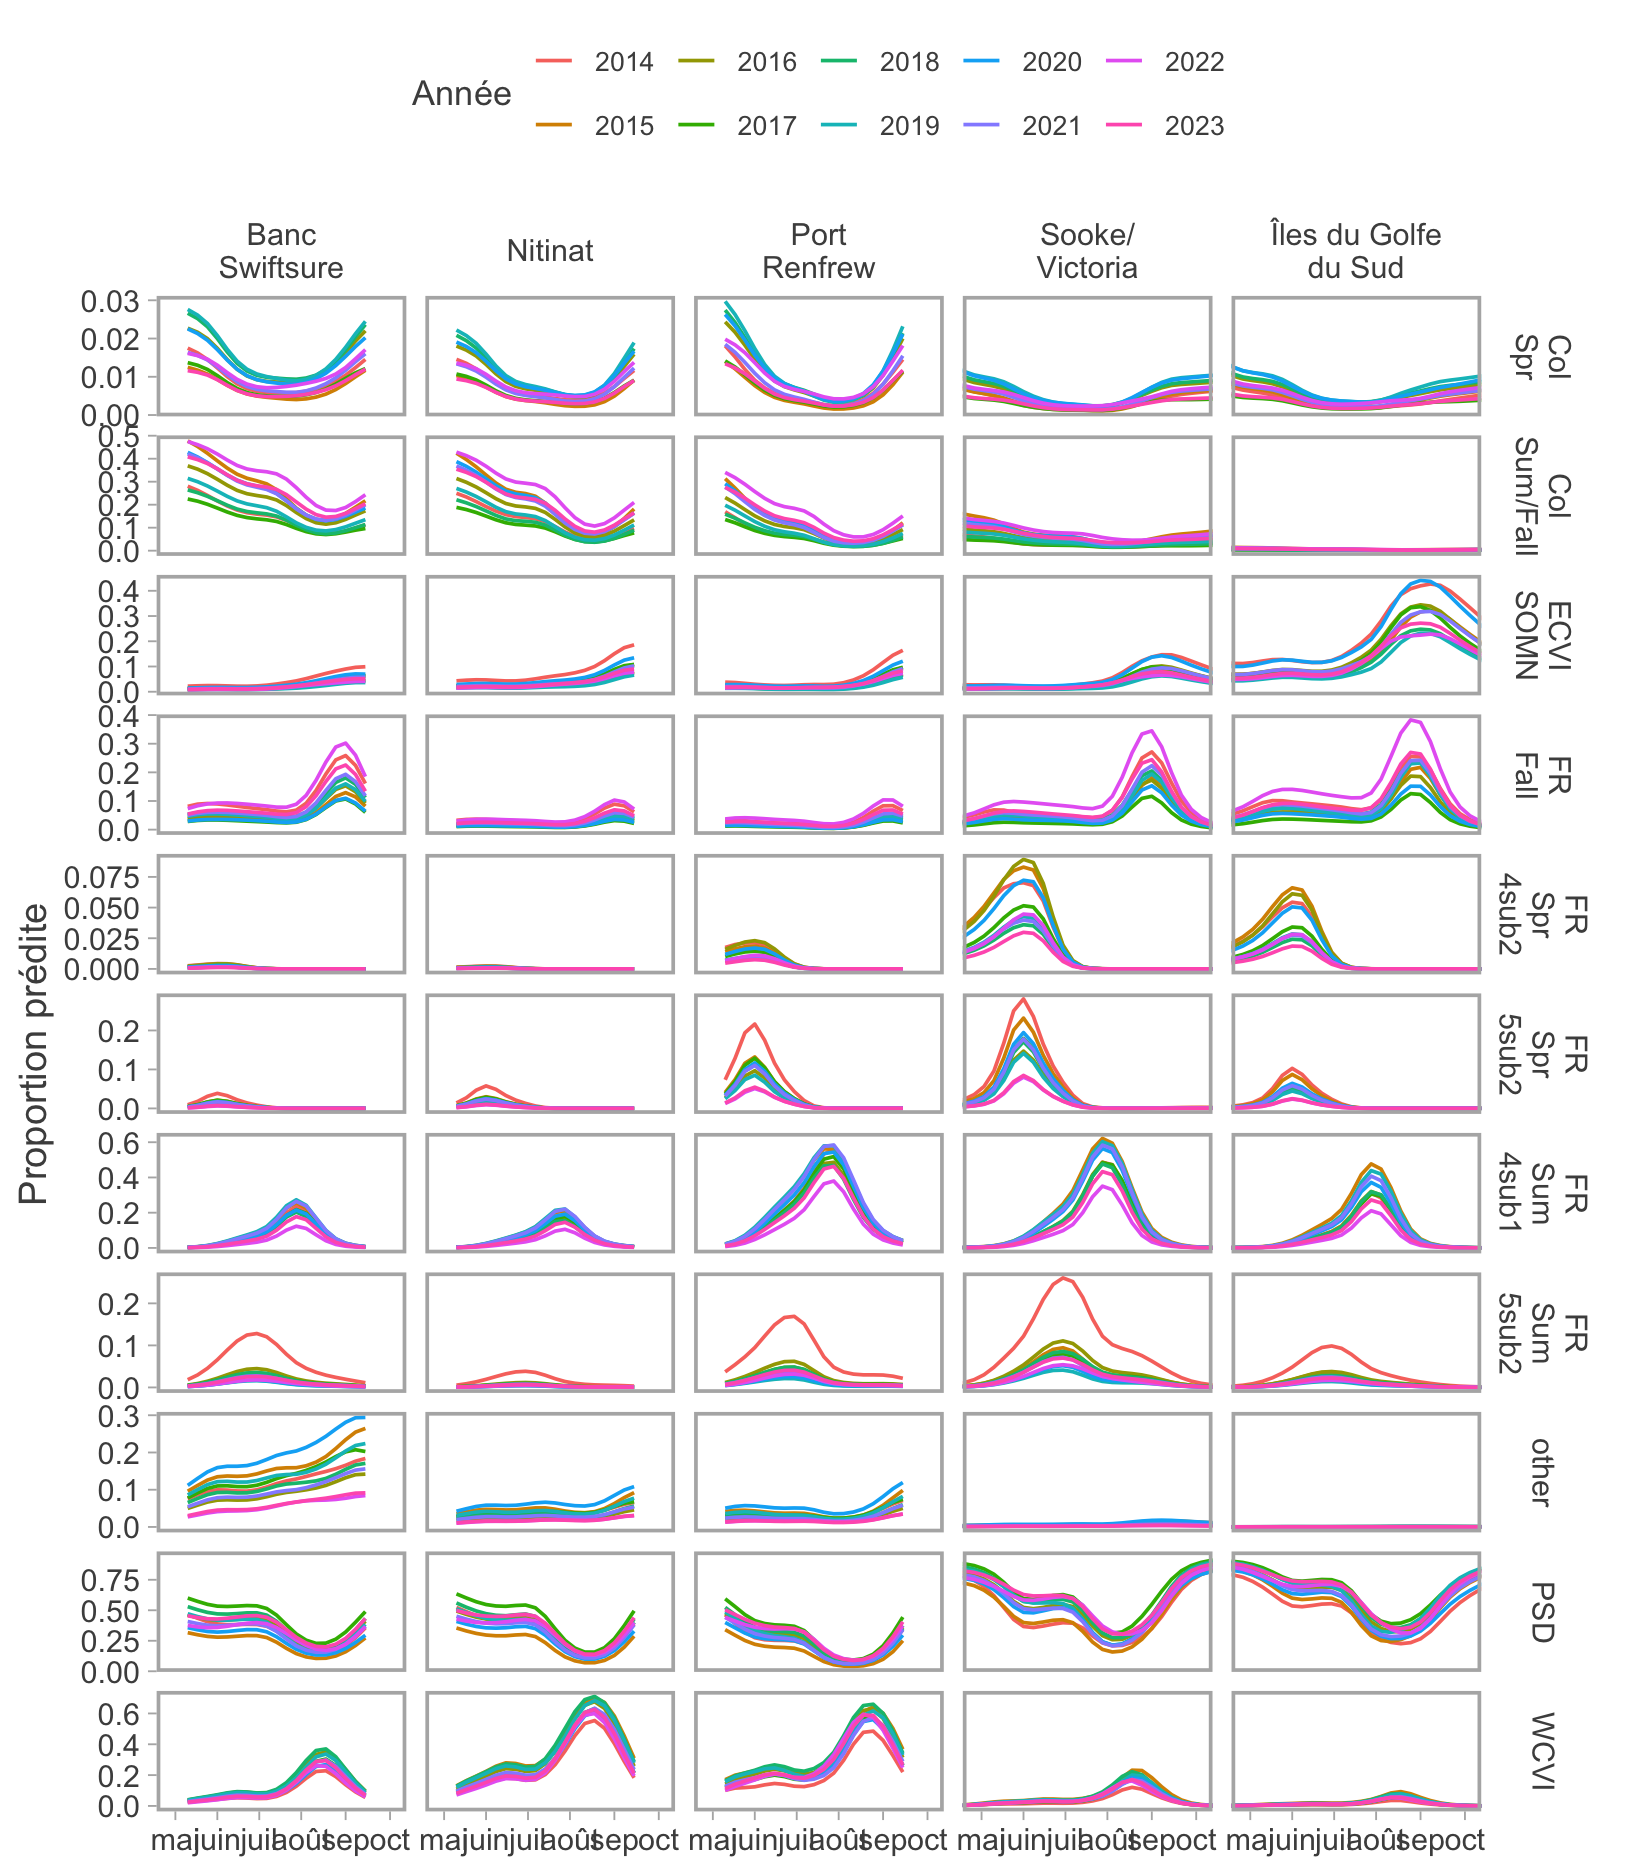
\includegraphics[width=5in]{figs/supp_figs/smooth_preds_chinook_year.png}}{Figure \ref{fig:smooth-pred-rec-year}}
    \caption{Composition moyenne prédite du stock spécifique à l'année. Les strates (panneaux) correspondent aux domaines spatiaux de la Figure \ref{fig:sampling-map}. Les intervalles de confiance ne sont pas montrés pour améliorer la lisibilité.}
    \label{fig:smooth-pred-rec-year}
\end{figure}

\begin{figure}[htb]
    \centering
    \pdftooltip{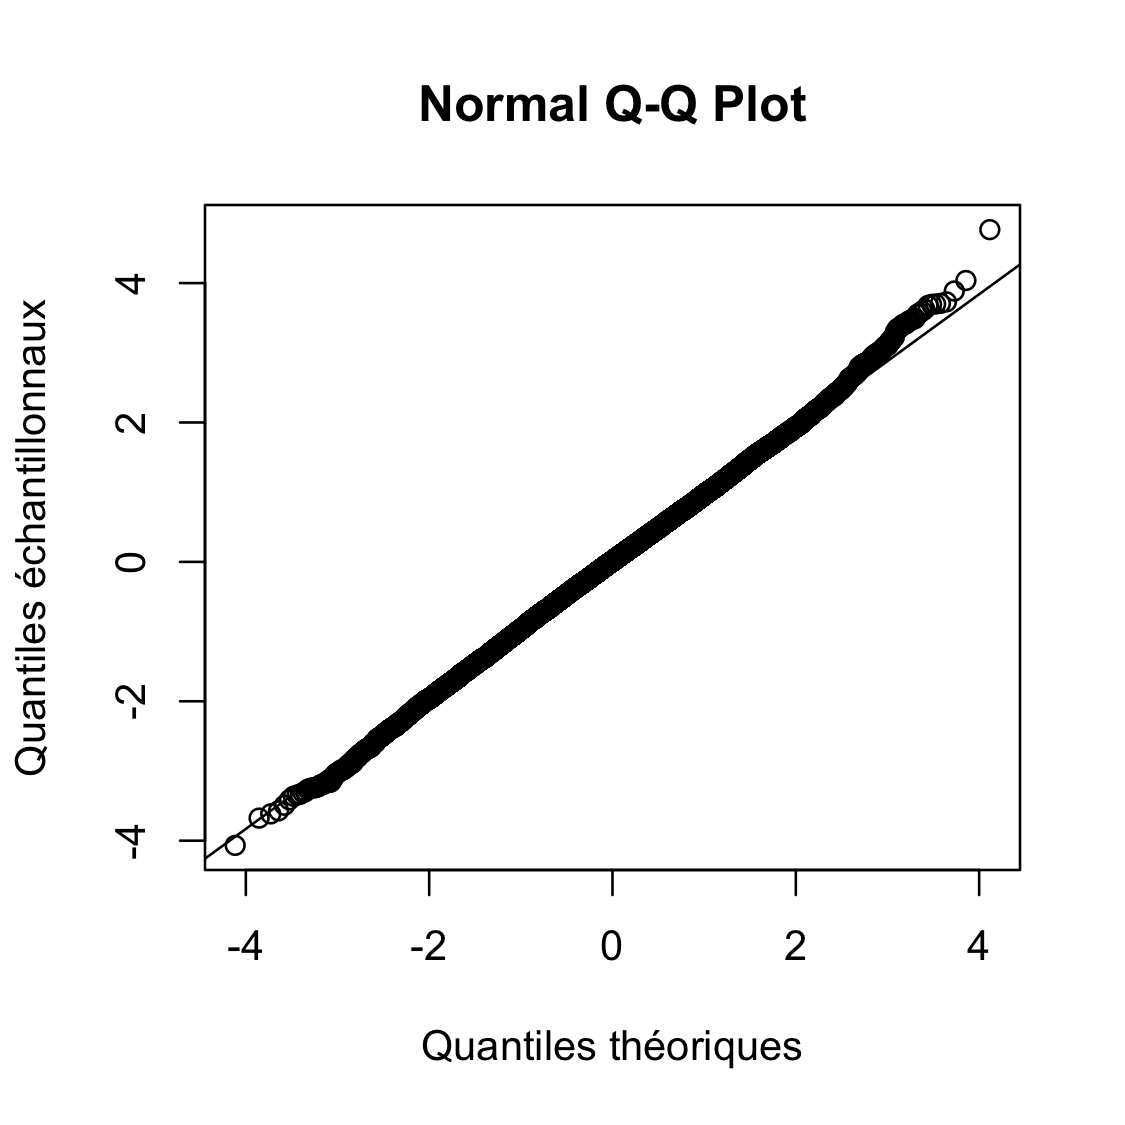
\includegraphics[width=5in]{figs/supp_figs/qq_plot_stock.png}}{Figure \ref{fig:qqplot-stock}}
    \caption{Résidus du modèle calculés à l'aide de tirages MCCM à partir de la distribution postérieure des prédictions avec des effets fixes aux estimations du maximum de vraisemblance et des effets aléatoires (c.-à-d., variance résiduelle) échantillonnés à partir de la distribution de Tweedie.}
    \label{fig:qqplot-stock}
\end{figure}

\begin{figure}[htb]
    \centering
    \pdftooltip{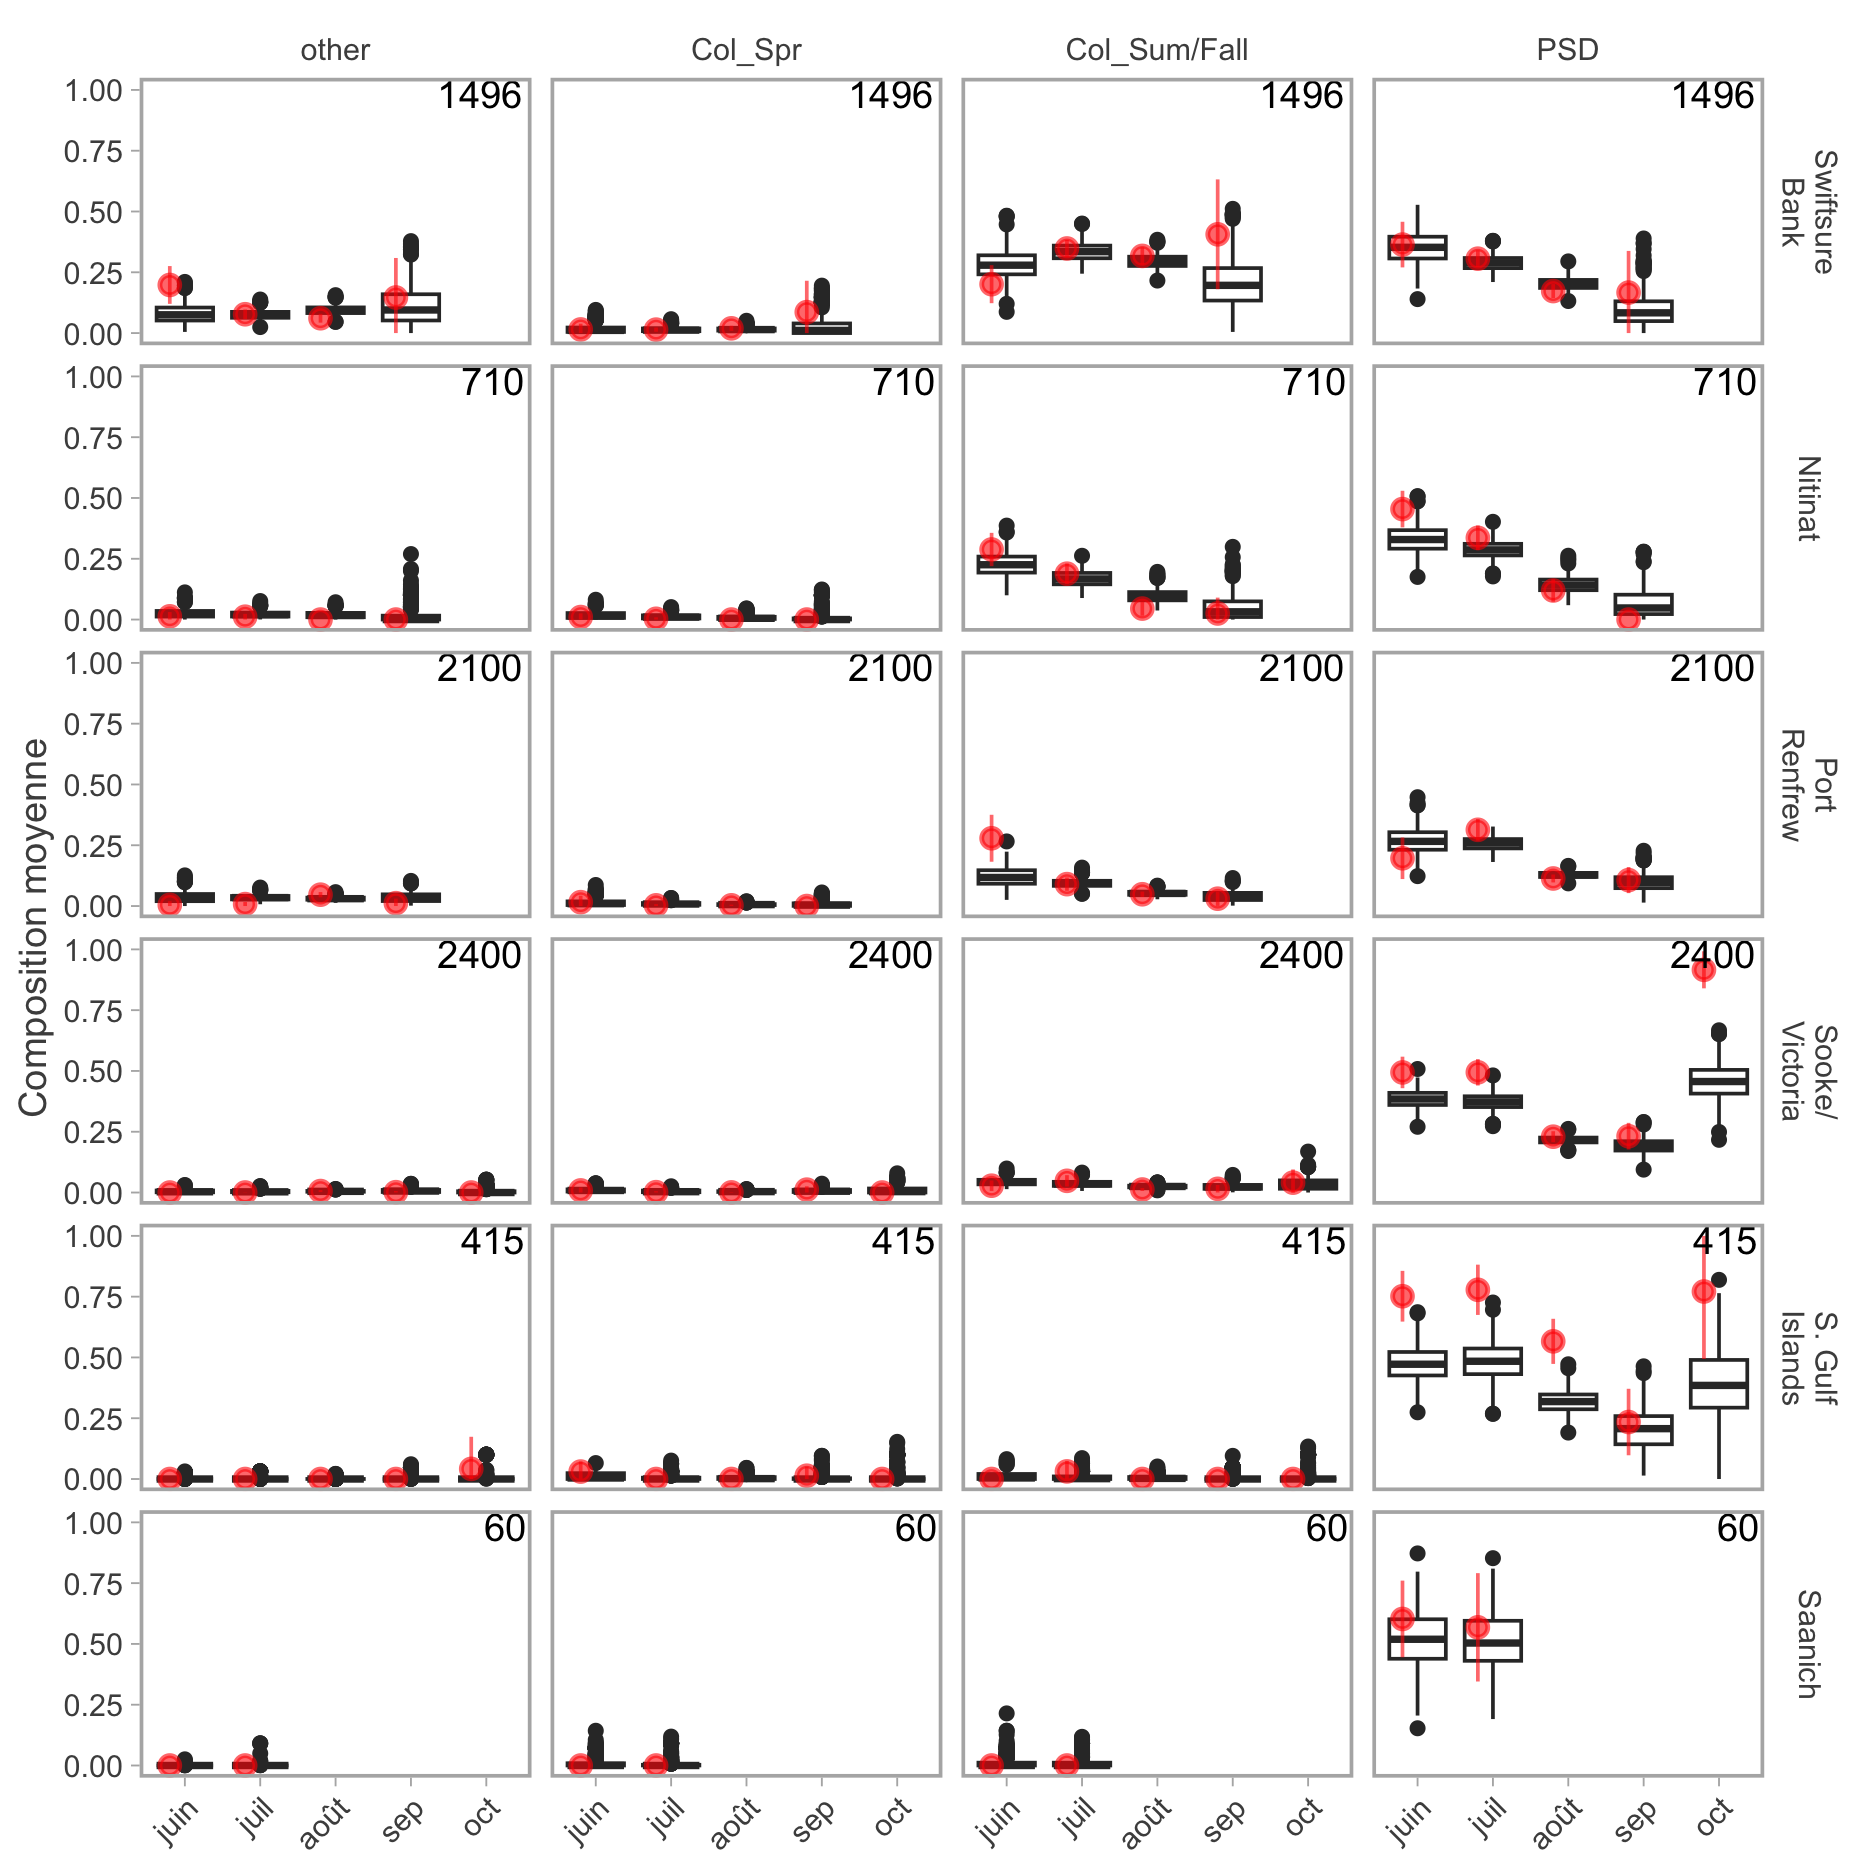
\includegraphics[width=5in]{figs/supp_figs/posterior_sims_stock1.png}}{Figure \ref{fig:posterior-stock1}}
    \caption{Composition moyenne simulée par modèle (diagrammes en boîte) et observée (points rouges) du stock pour les stocks «\,autre\,», Columbia Spring, Columbia Summer/Fall et Puget Sound. Les simulations représentent 500 tirages du modèle de Tweedie multivarié estimé, incluant la variance résiduelle, ajusté au jeu de données original. Les moustaches rouges représentent les intervalles de confiance approximatifs de 95\,\% associés à l'échantillon observé. Composition moyenne du stock calculée pour chaque strate et chaque mois. Les strates (panneaux) correspondent aux domaines spatiaux de la Figure \ref{fig:sampling-map}.}
    \label{fig:posterior-stock1}
\end{figure}

\begin{figure}[htb]
    \centering
    \pdftooltip{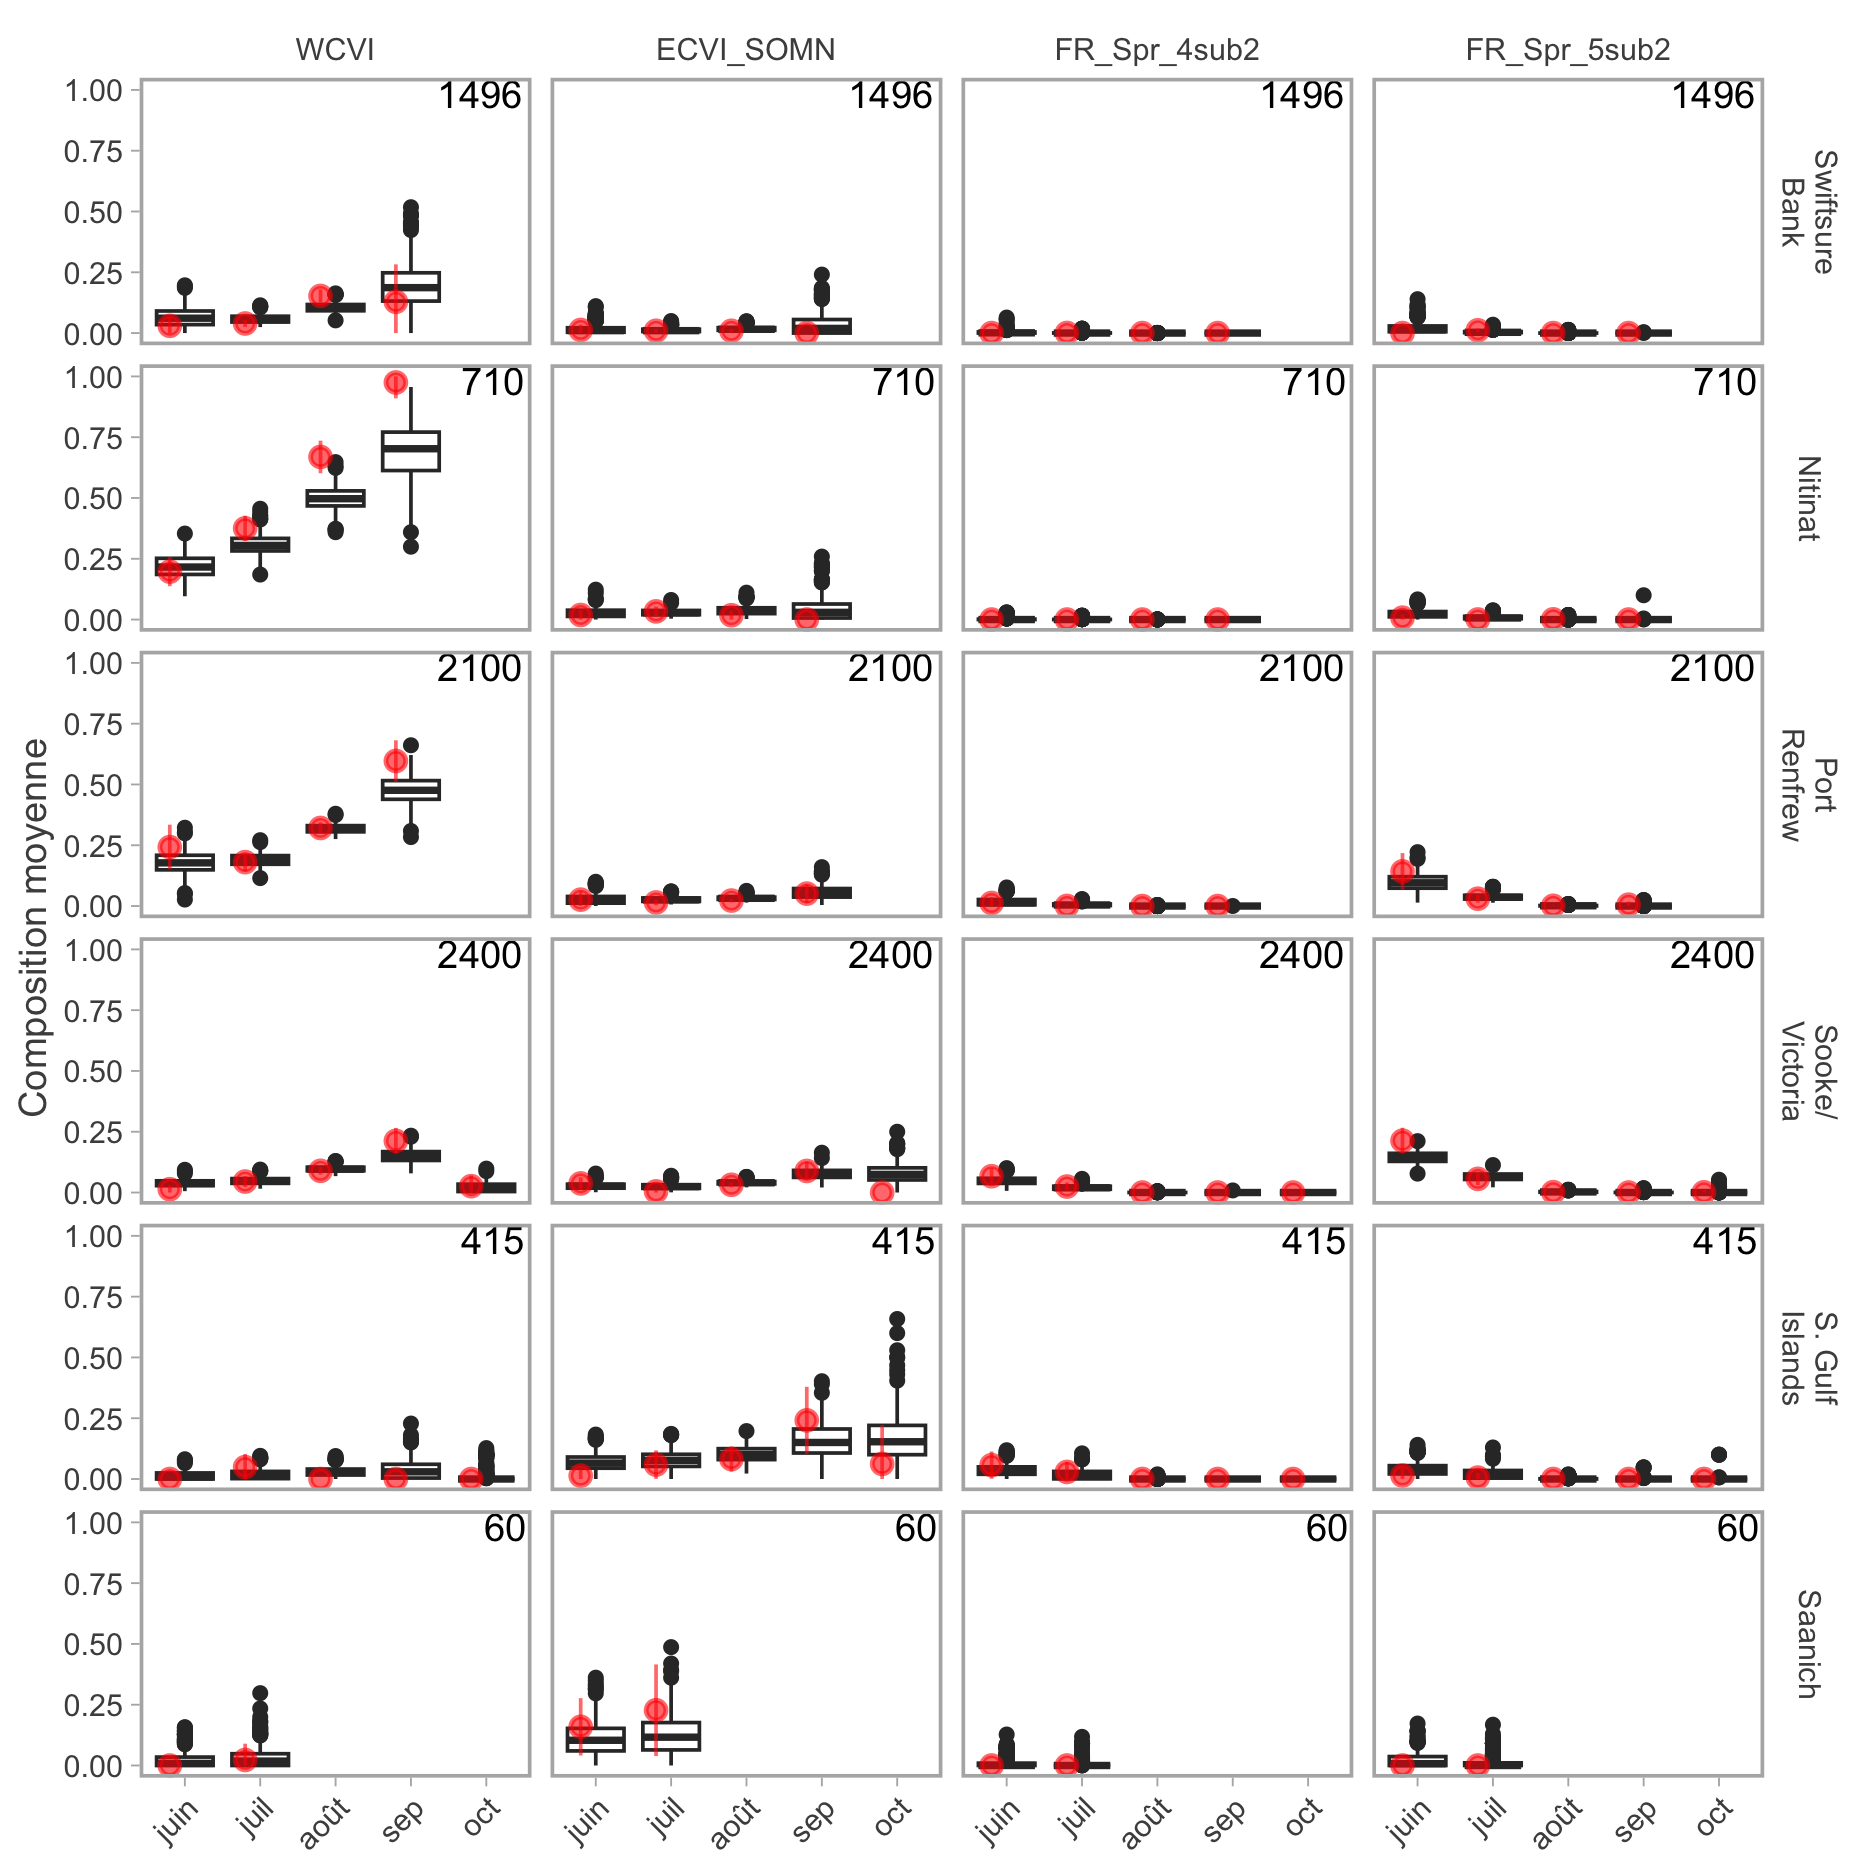
\includegraphics[width=5in]{figs/supp_figs/posterior_sims_stock2.png}}{Figure \ref{fig:posterior-stock2}}
    \caption{Composition moyenne simulée par modèle (diagrammes en boîte) et observée (points rouges) du stock pour les stocks de la côte ouest de l'île de Vancouver, de la côte est de l'île de Vancouver/continent méridional, Fraser Spring $4_2$ et Fraser Spring $5_2$. Les simulations représentent 500 tirages du modèle de Tweedie multivarié estimé, incluant la variance résiduelle, ajusté au jeu de données original. Les moustaches rouges représentent les intervalles de confiance approximatifs de 95\,\% associés à l'échantillon observé. Composition moyenne du stock calculée pour chaque strate et chaque mois. Les strates (panneaux) correspondent aux domaines spatiaux de la Figure \ref{fig:sampling-map}.}
    \label{fig:posterior-stock2}
\end{figure}

\begin{figure}[htb]
    \centering
    \pdftooltip{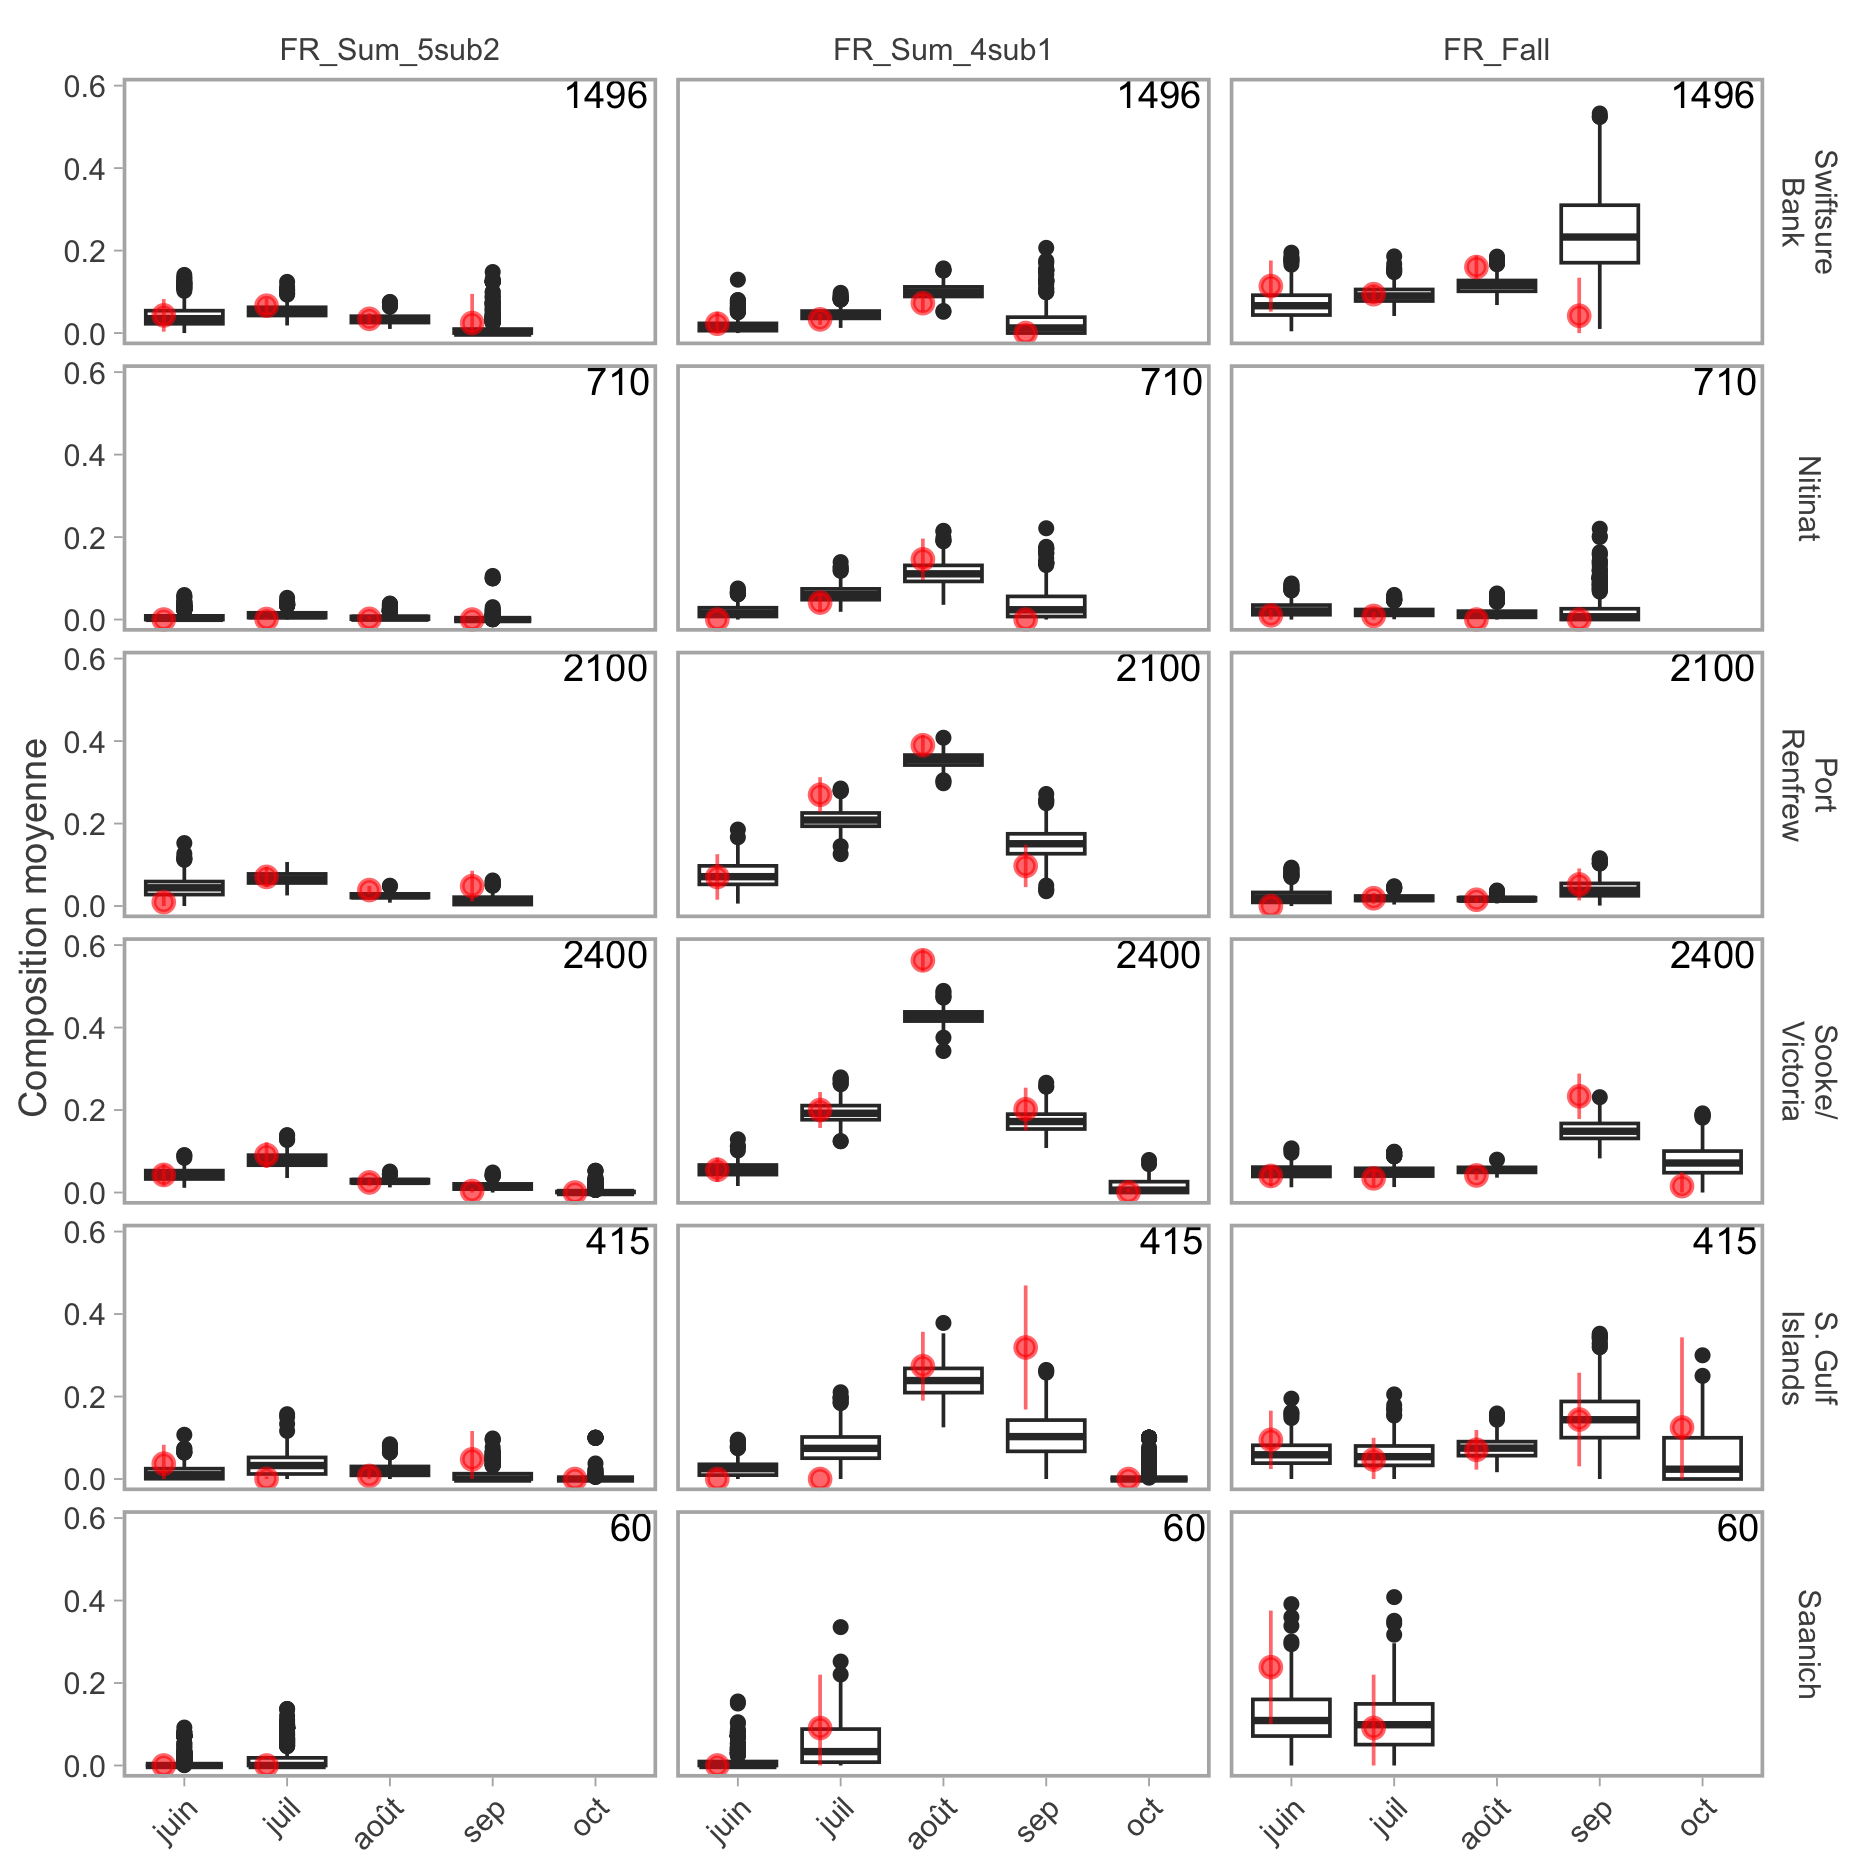
\includegraphics[width=5in]{figs/supp_figs/posterior_sims_stock3.png}}{Figure \ref{fig:posterior-stock3}}
    \caption{Composition moyenne simulée par modèle (diagrammes en boîte) et observée (points rouges) du stock pour les stocks Fraser Summer $5_2$, Fraser Summer $4_1$ et Fraser Fall. Les simulations représentent 500 tirages du modèle de Tweedie multivarié estimé, incluant la variance résiduelle, ajusté au jeu de données original. Les moustaches rouges représentent les intervalles de confiance approximatifs de 95\,\% associés à l'échantillon observé. Composition moyenne du stock calculée pour chaque strate et chaque mois. Les strates (panneaux) correspondent aux domaines spatiaux de la Figure \ref{fig:sampling-map}.}
    \label{fig:posterior-stock3}
\end{figure}

\begin{figure}[htb]
    \centering
    \pdftooltip{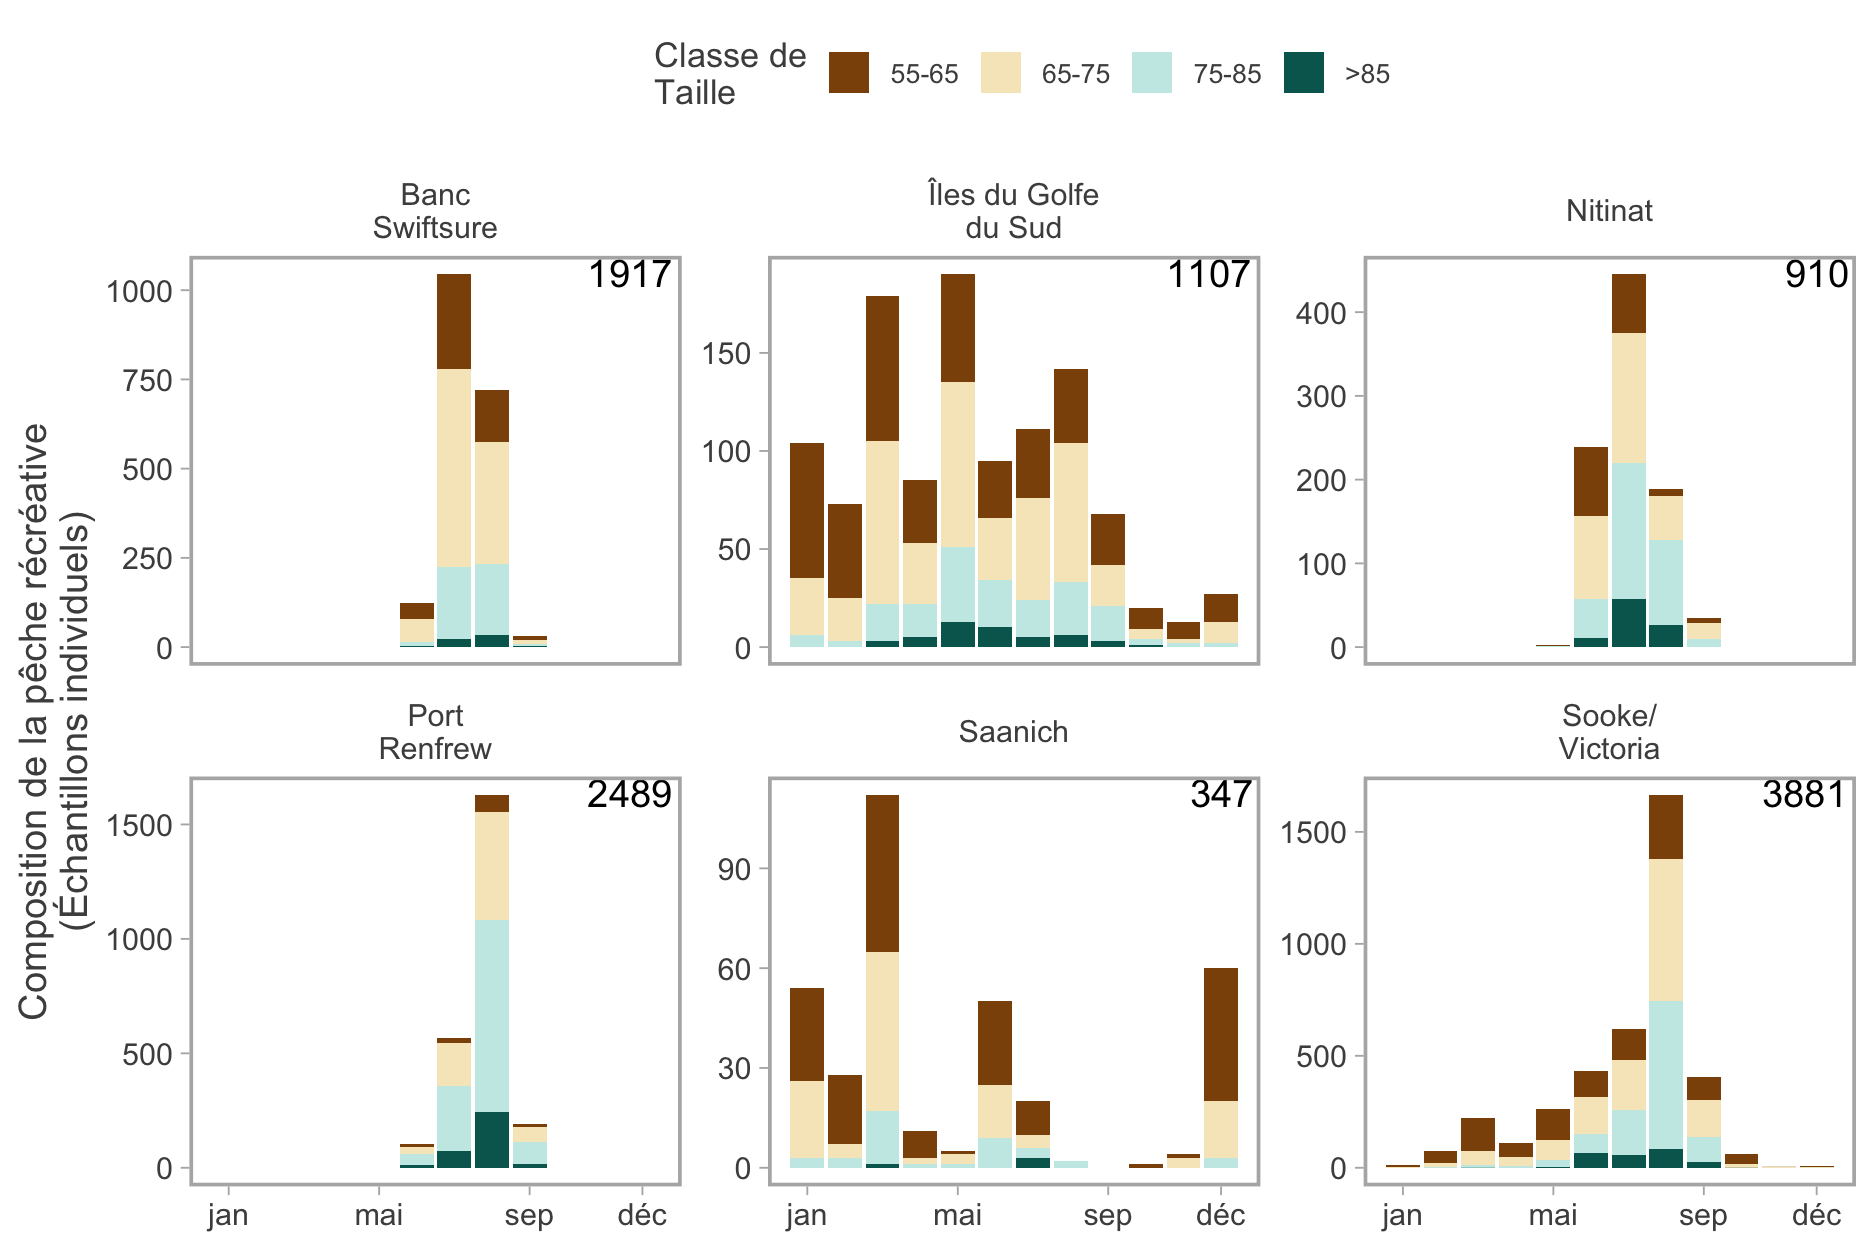
\includegraphics[width=5in]{figs/supp_figs/rec_monthly_size_bar.png}}{Figure \ref{fig:bar-rec-full-size}}
    \caption{Composition mensuelle de taille d'échantillons de la pêche récréative de saumon chinook pendant tous les mois. Les strates (panneaux) correspondent aux domaines spatiaux de la Figure \ref{fig:sampling-map}. L'axe des y représente le nombre d'échantillons collectés dans un mois et une strate spatiale donnés (notez que l'échelle diffère entre les strates). Les chiffres dans le coin supérieur droit de chaque panneau représentent la taille totale de l'échantillon dans chaque strate.}
    \label{fig:bar-rec-full-size}
\end{figure}

\begin{figure}[htb]
    \centering
    \pdftooltip{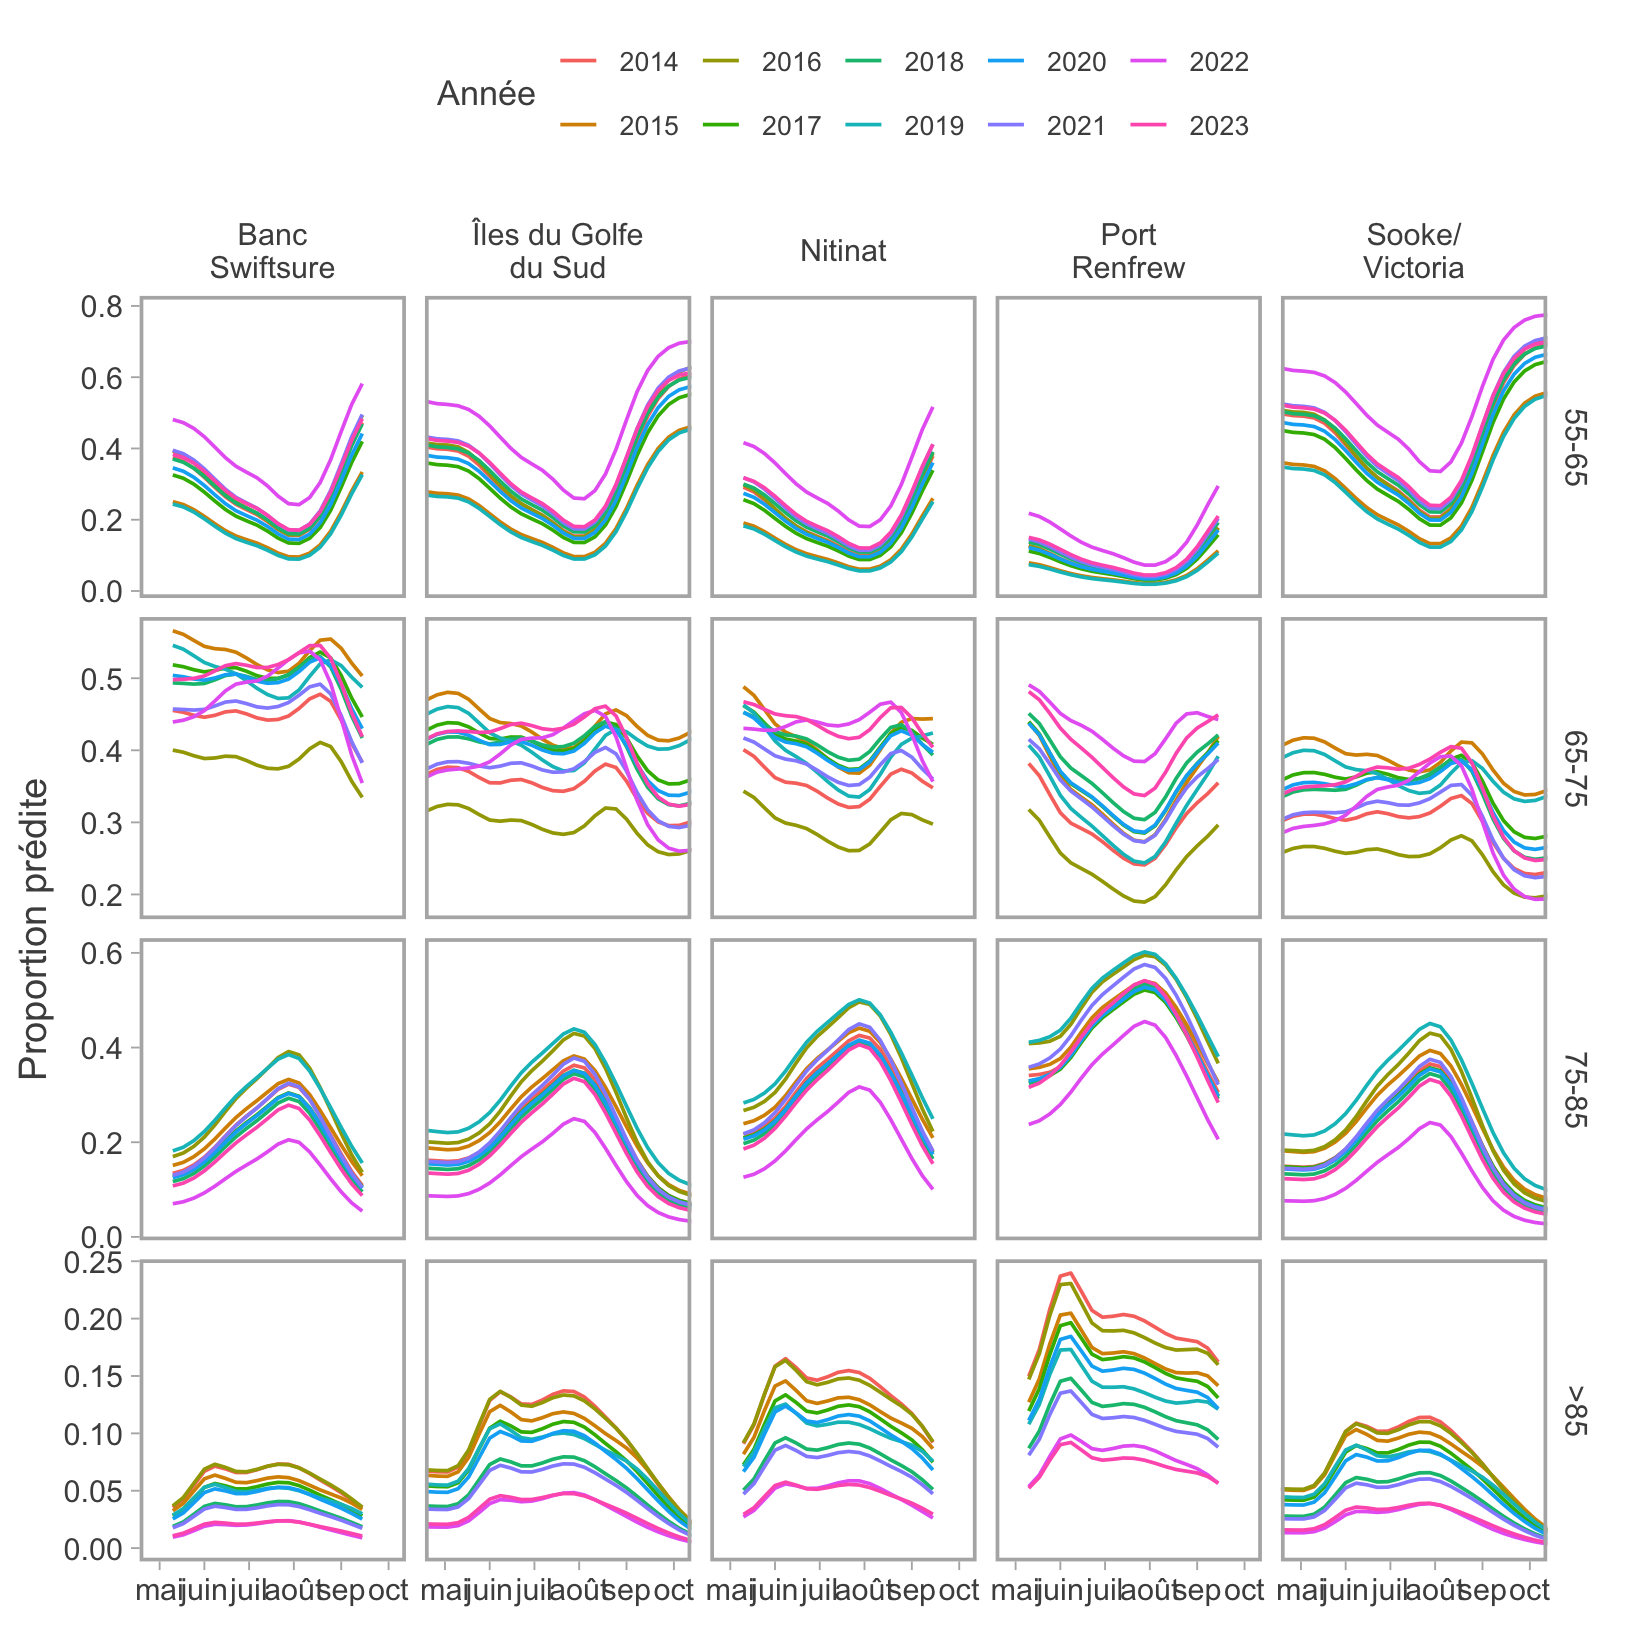
\includegraphics[width=5in]{figs/supp_figs/size_smooth_preds_chinook_year.png}}{Figure \ref{fig:size-smooth-pred-rec-year}}
    \caption{Composition moyenne prédite de taille spécifique à l'année. Les strates (panneaux) correspondent aux domaines spatiaux de la Figure \ref{fig:sampling-map}. Les intervalles de confiance ne sont pas montrés pour améliorer la lisibilité.}
    \label{fig:size-smooth-pred-rec-year}
\end{figure}

\begin{figure}[htb]
    \centering
    \pdftooltip{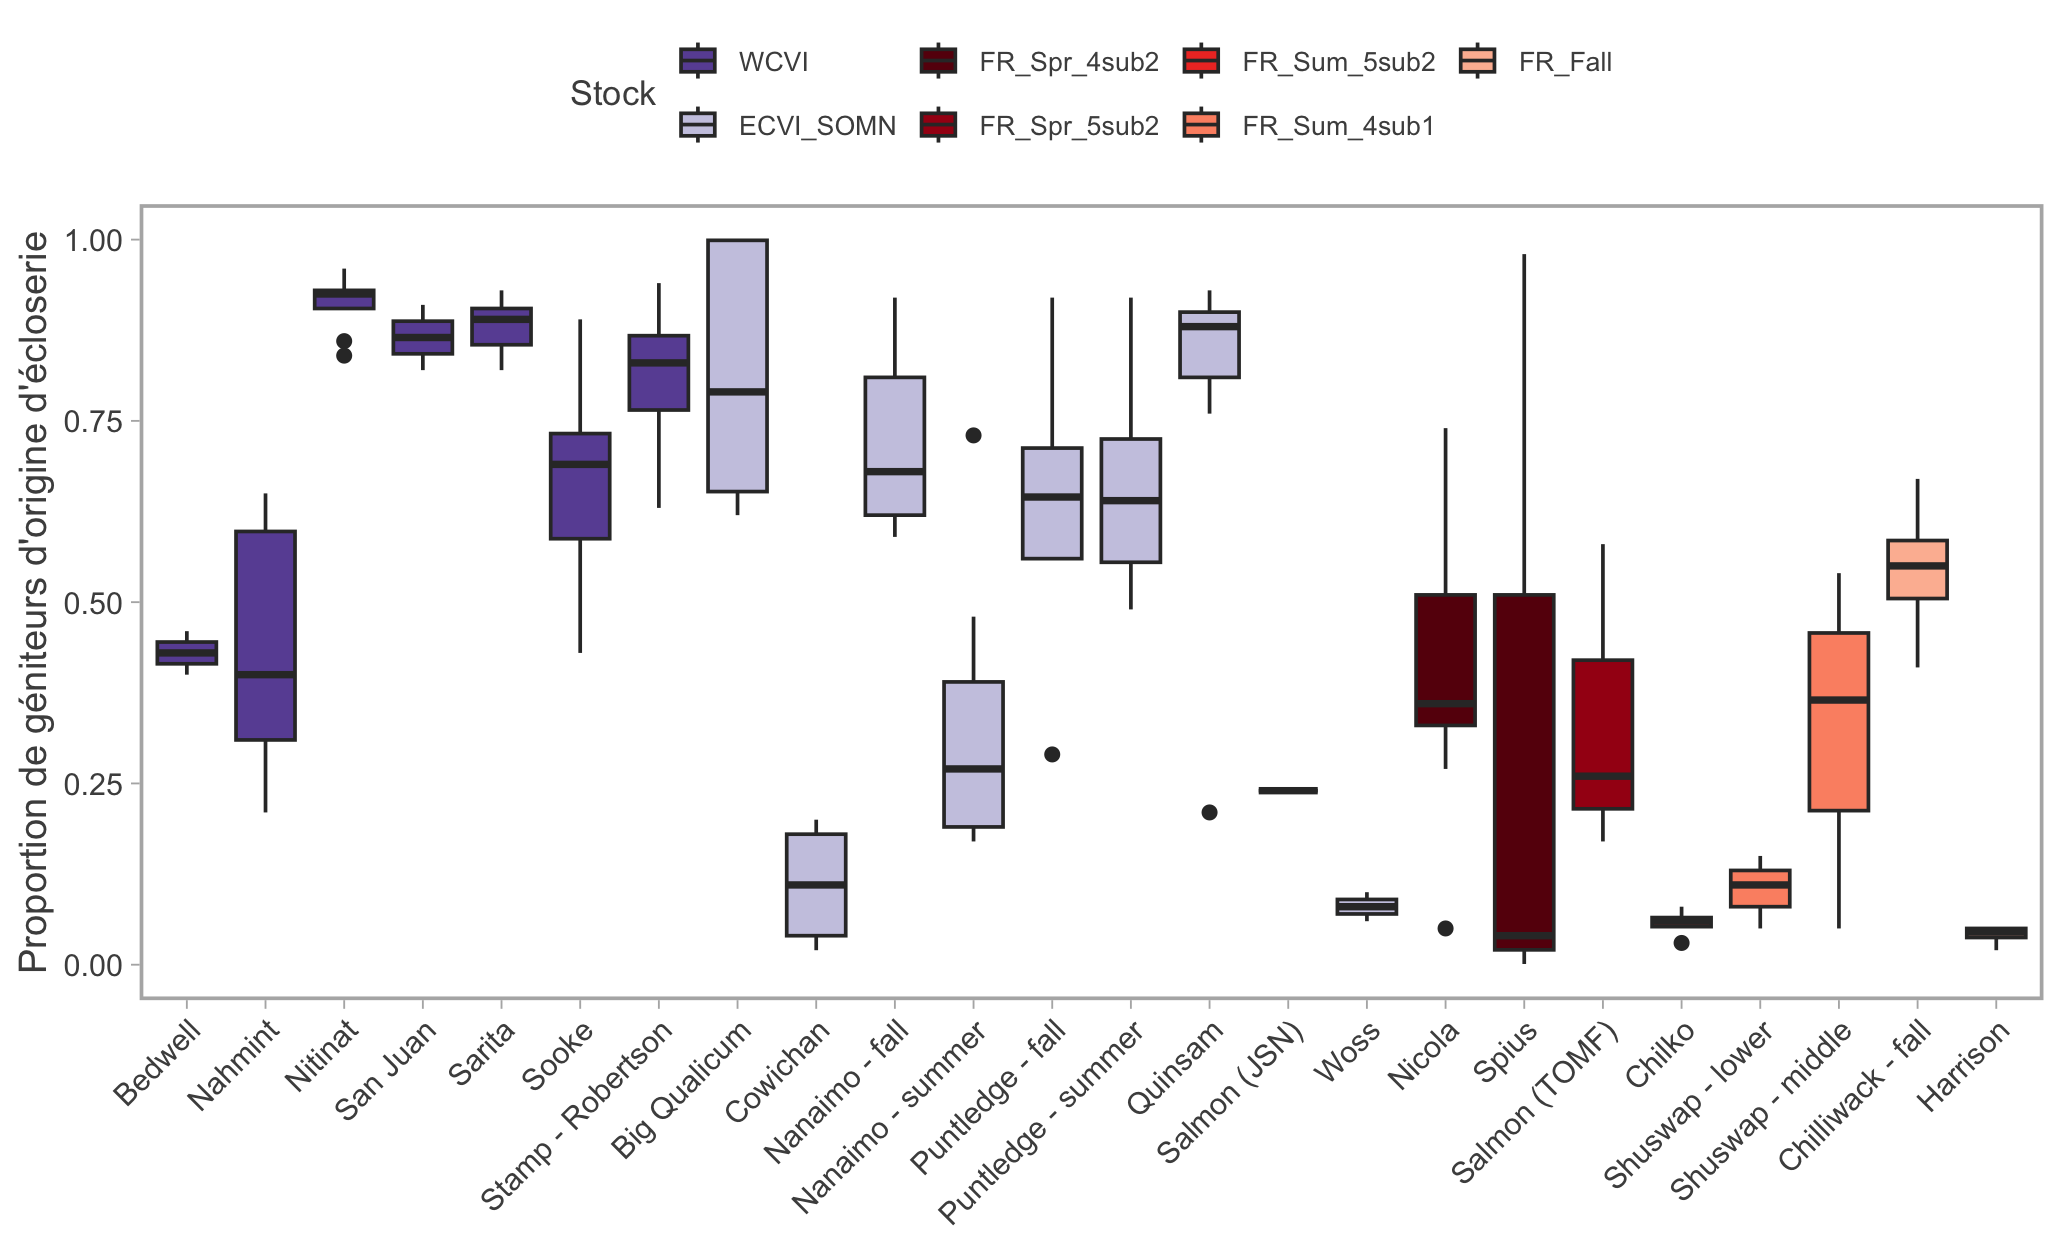
\includegraphics[width=5in]{figs/supp_figs/phos_box.png}}{Figure \ref{fig:box-phos}}
    \caption{La proportion estimée de géniteurs d'origine d'écloserie pour un sous-ensemble de populations de saumon chinook canadiennes. Les diagrammes en boîte représentent la variabilité entre les années (2014-2022). Les couleurs représentent les stocks d'origine canadienne.}
    \label{fig:box-phos}
\end{figure}

\begin{figure}[htb]
    \centering
    \pdftooltip{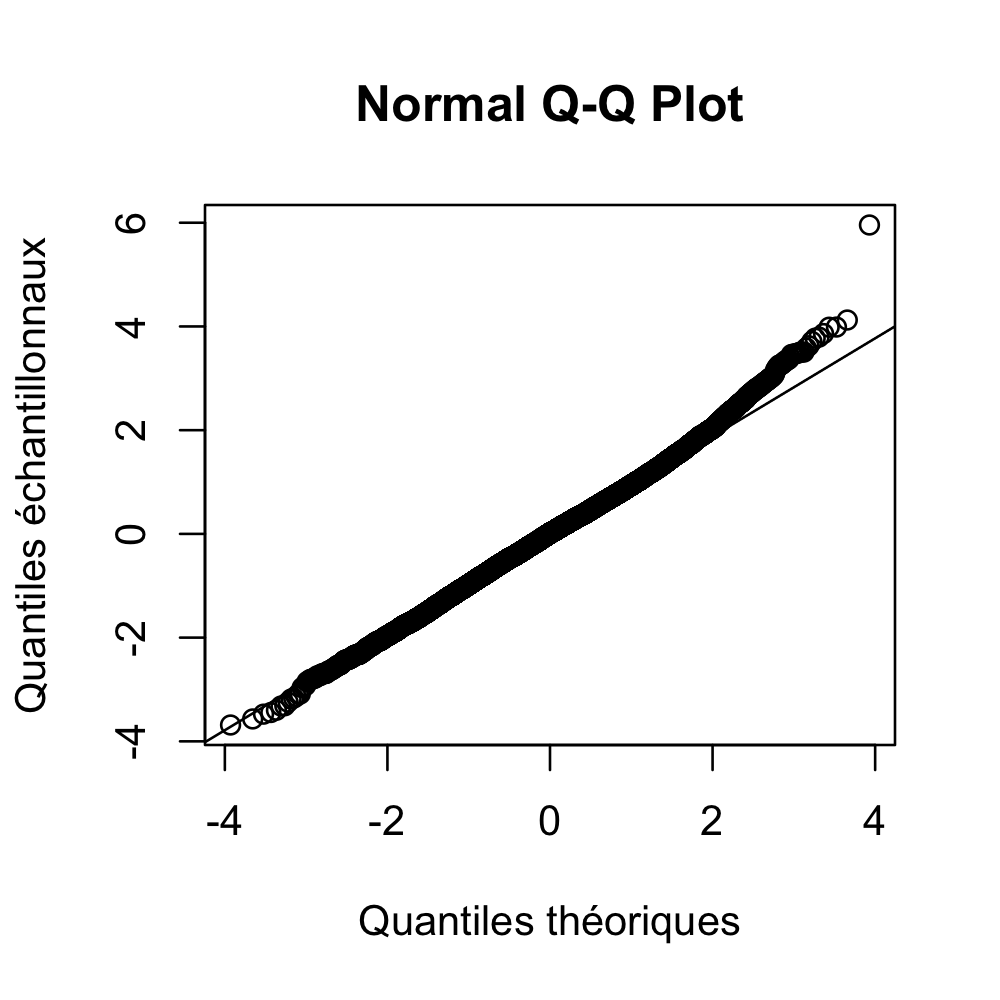
\includegraphics[width=5in]{figs/supp_figs/qq_plot_size.png}}{Figure \ref{fig:qqplot-size}}
    \caption{Graphique quantile-quantile des résidus du modèle de composition de taille calculés à l'aide de tirages MCCM à partir de la distribution postérieure des prédictions avec des effets fixes fixés aux estimations du maximum de vraisemblance et des effets aléatoires (c.-à-d., variance résiduelle) échantillonnés à partir de la distribution binomiale négative.}
    \label{fig:qqplot-size}
\end{figure}

\begin{figure}[htb]
    \centering
    \pdftooltip{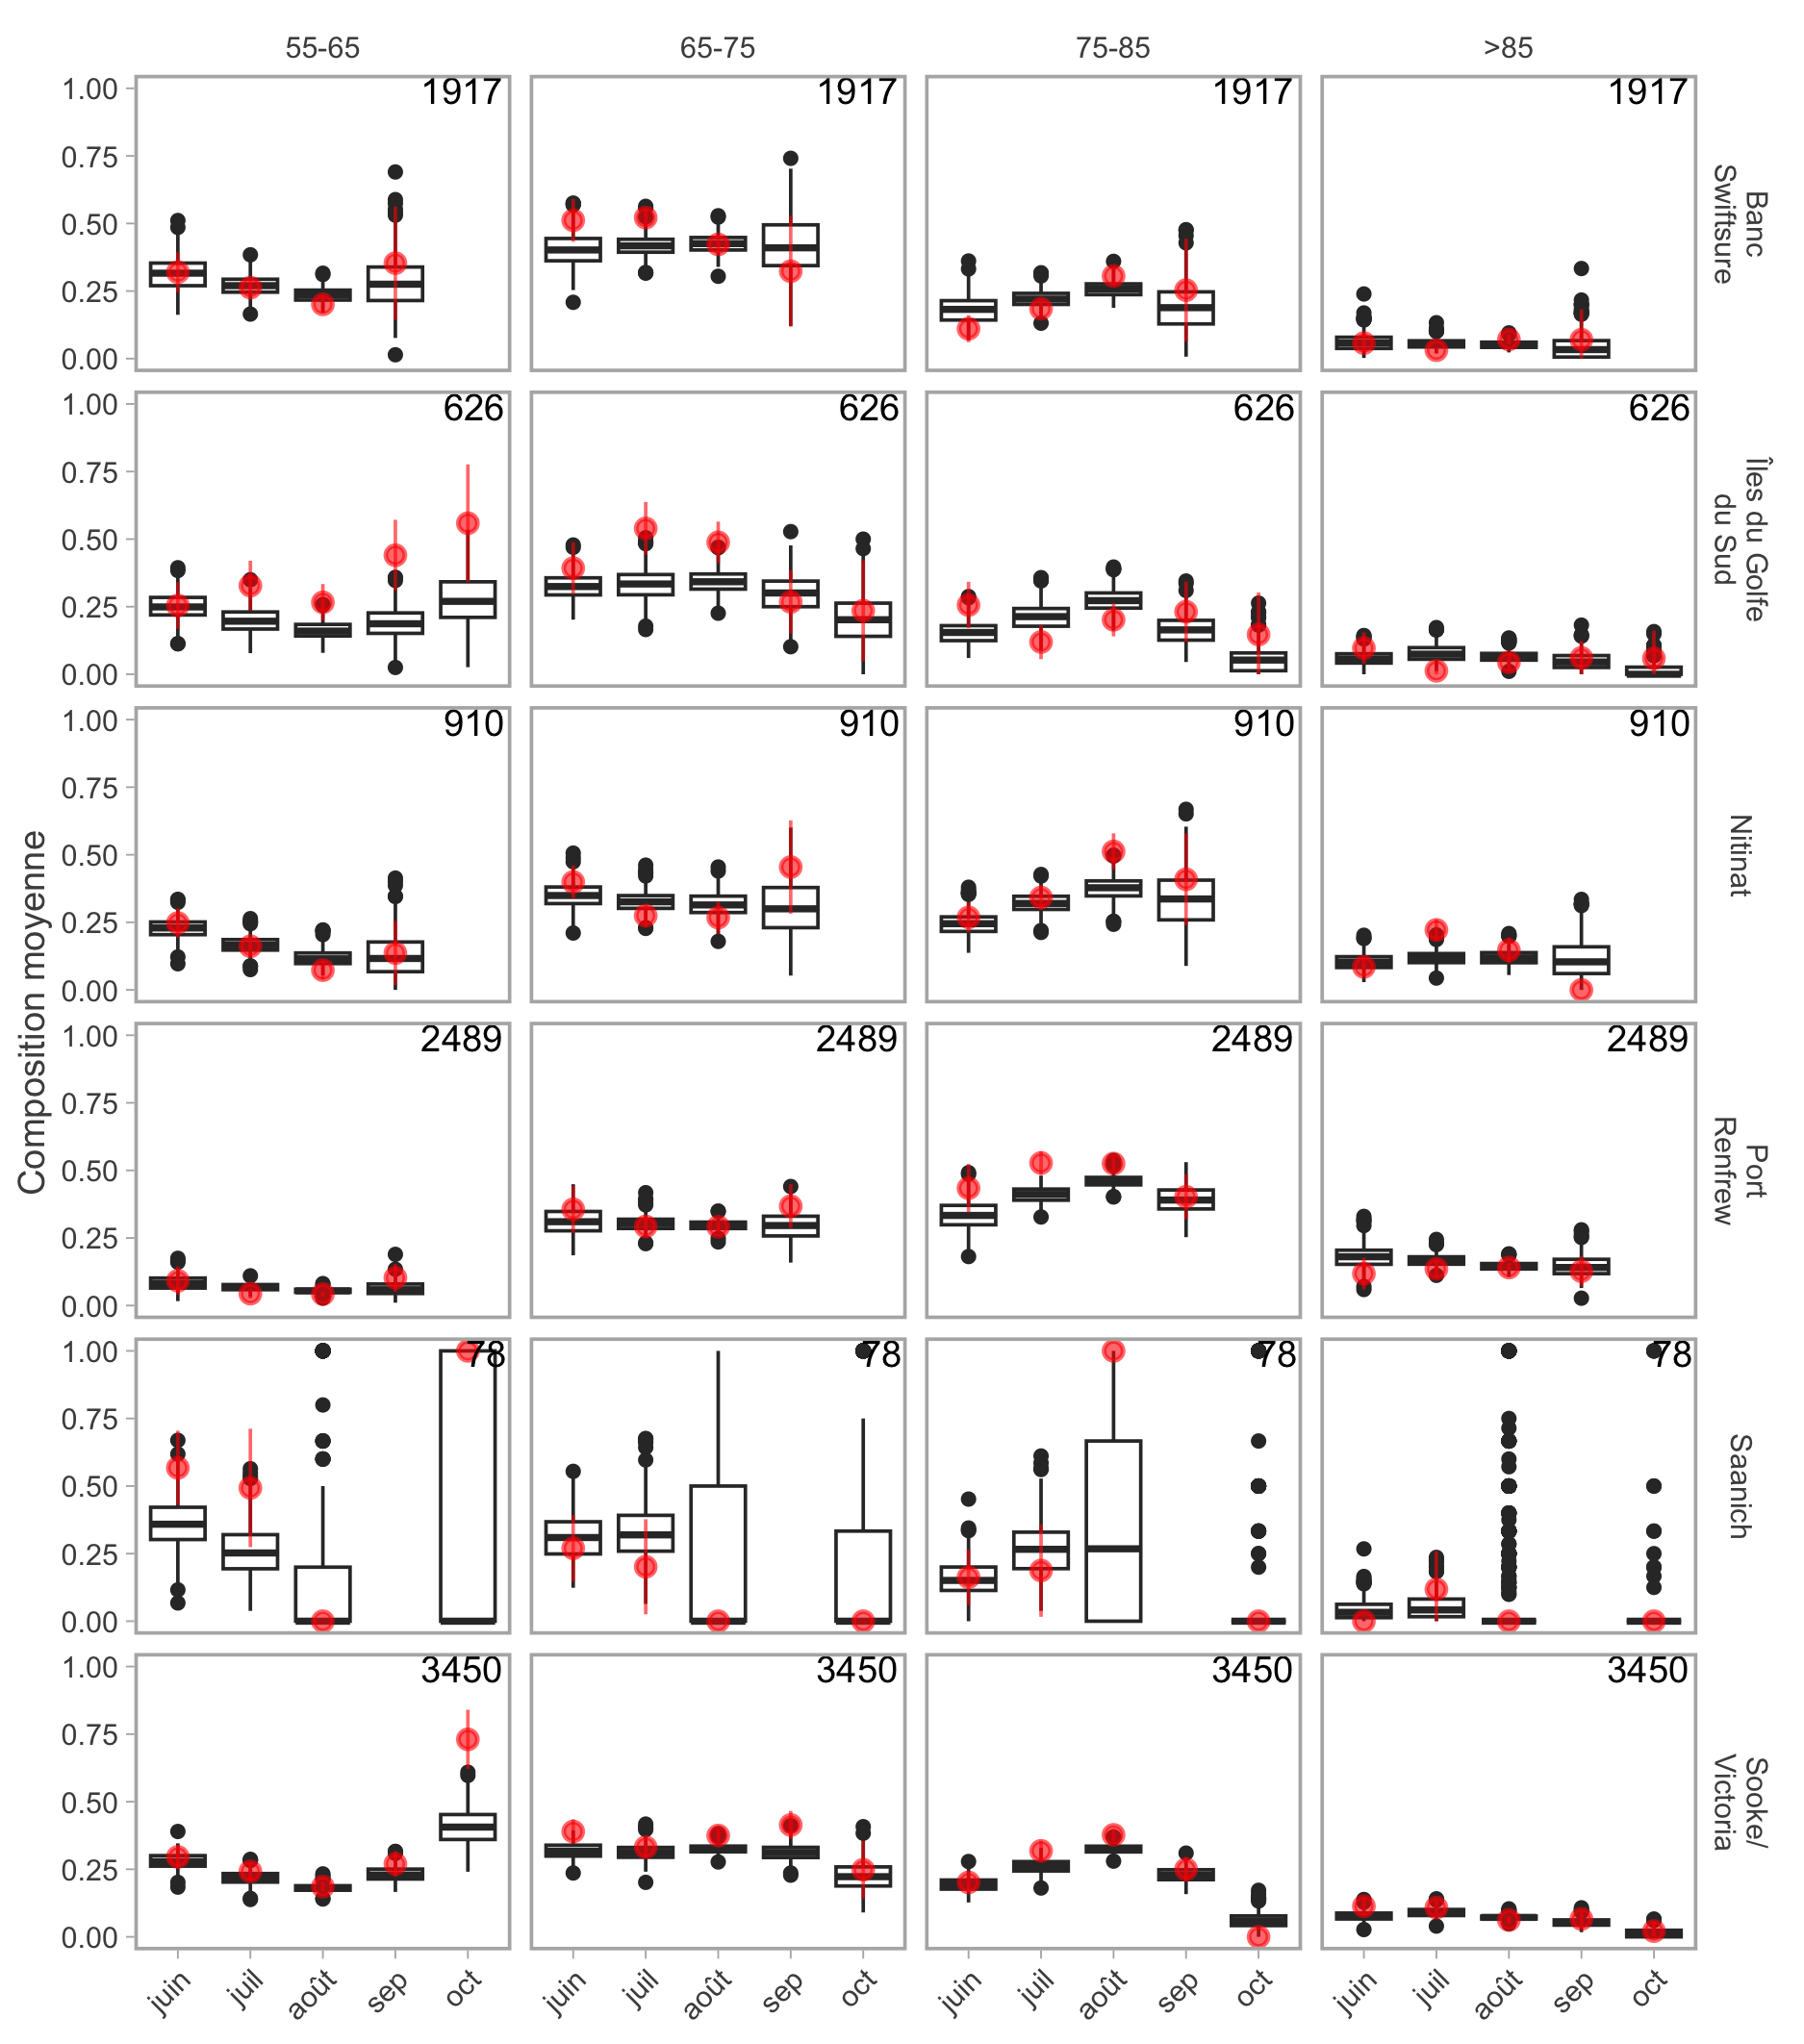
\includegraphics[width=5in]{figs/supp_figs/posterior_sims_size.png}}{Figure \ref{fig:posterior-size}}
    \caption{Composition moyenne simulée par modèle (diagrammes en boîte) et observée (points rouges) du stock. Les simulations représentent 500 tirages du modèle de Tweedie estimé, incluant la variance résiduelle, ajusté au jeu de données original. Les moustaches rouges représentent les intervalles de confiance approximatifs de 95\,\% associés à l'échantillon observé. Composition moyenne du stock calculée pour chaque strate et chaque mois. Les strates (panneaux) correspondent aux domaines spatiaux de la Figure \ref{fig:sampling-map}.}
    \label{fig:posterior-size}
\end{figure}
